\mfpicnumber{1}

\opengraphsfile{LogarithmicFunctions}

\setcounter{footnote}{0}

\label{LogarithmicFunctions}


In Section \ref{ExponentialFunctions}, we saw exponential functions $f(x) = b^x$  are are one-to-one which means they are invertible.   In this section, we explore their inverses, the \textit{logarithmic functions} which are called `logs' for short.

\smallskip

\colorbox{ResultColor}{\bbm

\begin{defn} \label{logfcndefn} For the exponential function $f(x) = b^{x}$,  $f^{-1}(x) = \log_{b}(x)$ is called the \index{function ! logarithmic} \textbf{base \boldmath $b$ logarithm function}.  We read `$\log_{b}(x)$' as `log base $b$ of $x$.' \index{logarithm ! general, ``base $b$''}

\end{defn}

\ebm}
\smallskip

We have special notations for the common base, $b=10$, and the natural base, $b=e$.


\smallskip

\colorbox{ResultColor}{\bbm

\begin{defn} $~$

\begin{itemize}

\item  The \index{logarithm ! common} \textbf{common logarithm} of a real number $x$ is $\log_{10}(x)$ and is usually written $\log(x)$.   

\item The \index{logarithm ! natural} \textbf{natural logarithm} of a real number $x$ is $\log_{e}(x)$ and is usually written $\ln(x)$. \index{common logarithm} \index{natural logarithm}

\end{itemize}

\end{defn}

\ebm}
\smallskip

Since logs are defined as the inverses of exponential functions, we can use Theorems \ref{inversefunctionprops} and \ref{expfcnprops} to tell us about logarithmic functions.  For example, we know that the domain of a log function is the range of an exponential function, namely $(0, \infty)$, and that the range of a log function is the domain of an exponential function, namely $(-\infty, \infty)$.   

\smallskip

Moreover, since we know the basic shapes of $y = f(x) = b^{x}$ for the different cases of $b$, we can obtain the graph of $y = f^{-1}(x) = \log_{b}(x)$ by reflecting the graph of $f$ across the line $y=x$.  The $y$-intercept $(0,1)$ on the graph of $f$  corresponds to an $x$-intercept of $(1,0)$ on the graph of $f^{-1}$.  The horizontal asymptotes $y=0$ on the graphs of the exponential functions become vertical asymptotes $x=0$ on the log graphs.  

\[ \begin{array}{cc}

\begin{mfpic}[15]{-3}{5}{-3}{5}
\axes
\tlabel[cc](5,-0.5){\scriptsize $x$}
\tlabel[cc](0.5,5){\scriptsize $y$}
\xmarks{1}
\ymarks{1}
\arrow \reverse \arrow \function{-2.3, 2.3, 0.1}{2**x}
\point[2pt]{(0,1)}
\dashed \polyline{(-1,-1), (5,5)}
\tlabel[cc](3,-4){\scriptsize $y =b^{x}$, $b > 1$}
\tlabel[cc](-1.5,1){\scriptsize $(0,1)$}
\tlabel[cc](1.5,-0.5){\scriptsize \text{\boldmath $(0,1)$}}
\tlabel[cc](3,-5){\scriptsize \mbox{\boldmath $y = \log_{b}(x)$}, $b > 1$}
\penwd{1.5pt}
\arrow \reverse \arrow \parafcn{-2.3,2.3,0.1}{(2^t,t)}
\point[4pt]{(1,0)}
\end{mfpic}

& 

\hspace{1.5in}

\begin{mfpic}[15]{-3}{5}{-3}{5}
\axes
\tlabel[cc](5,-0.5){\scriptsize $x$}
\tlabel[cc](0.5,5){\scriptsize $y$}
\xmarks{1}
\ymarks{1}
\arrow \reverse \arrow \function{-2.3, 2.3, 0.1}{(0.5)**x}
\point[2pt]{(0,1)}
\tlabel[cc](-1.5,1){\scriptsize $(0,1)$}
\tlabel[cc](0.75,-0.75){\scriptsize \text{\boldmath $(0,1)$}}
\dashed \polyline{(-1,-1), (5,5)}
\tlabel[cc](3,-4){\scriptsize $y =b^{x}$, $0 < b < 1$}
\tlabel[cc](3,-5){\scriptsize \mbox{\boldmath $y = \log_{b}(x)$}, $0 < b < 1$}
\penwd{1.5pt}
\arrow \reverse \arrow \parafcn{-2.3,2.3,0.1}{(2^t,-t)}
\point[4pt]{(1,0)}
\end{mfpic}

\end{array}\]

Procedurally,  logarithmic functions  `undo' the exponential functions.  Consider the function $f(x) = 2^{x}$.  When we evaluate $f(3) = 2^{3} = 8$, the input $3$ becomes the exponent on the base $2$ to produce the real number $8$.  The function $f^{-1}(x) = \log_{2}(x)$ then takes the number $8$ as its input and returns the exponent $3$ as its output.  In symbols, $\log_{2}(8) = 3$. 

\smallskip

More generally, $\log_{2}(x)$ is the exponent you put on $2$ to get $x$.  Thus, $\log_{2}(16) = 4$, because $2^{4} = 16$.  The following theorem summarizes the basic properties of logarithmic functions, all of which come from the fact that they are inverses of exponential functions. 
\smallskip

\colorbox{ResultColor}{\bbm

\begin{thm} \label{logfcnprops} \textbf{Properties of Logarithmic Functions:} Suppose $f(x) = \log_{b}(x)$. \index{logarithm ! graphical properties of}

\begin{itemize}

\item  The domain of $f$ is $(0, \infty)$ and the range of $f$ is $(-\infty, \infty)$.

\item  $(1,0)$ is on the graph of $f$ and $x=0$ is a vertical asymptote of the graph of $f$.

\item  $f$ is one-to-one, continuous and smooth

\item  $b^{a} = c$ if and only if $\log_{b}(c) = a$.  That is, $\log_{b}(c)$ is the exponent you put on $b$ to obtain $c$.

\item  $\log_{b} \left(b^{x}\right) = x$ for all real numbers $x$ and $b^{\log_{b}(x)} = x$ for all $x > 0$

\end{itemize}

\begin{tabular}{m{2.5in}m{2.5in}}

\begin{itemize}

\item  If $b > 1$:

\begin{itemize}

\item  $f$ is always increasing

\item  As $x \rightarrow 0^{+}$, $f(x) \rightarrow -\infty$

\item  As $x \rightarrow \infty$, $f(x) \rightarrow \infty$

\item  The graph of $f$ resembles:

\begin{center}

\begin{mfpic}[10]{-1}{5}{-3}{3}
\axes
\xmarks{1}
\penwd{1.25pt}
\arrow \reverse \arrow \parafcn{-2.3,2.3,0.1}{(2^t,t)}
\tlabel[cc](1.75,-0.75){\scriptsize $(1,0)$}
\point[4pt]{(1,0)}
\tlabel[cc](3,-4){\scriptsize $y = \log_{b}(x)$, $b > 1$}
\end{mfpic}

\end{center}

\end{itemize}

\end{itemize}

&
\begin{itemize}

\item  If $0<b<1$:

\begin{itemize}

\item  $f$ is always decreasing

\item  As $x \rightarrow 0^{+}$, $f(x) \rightarrow \infty$

\item  As $x \rightarrow \infty$, $f(x) \rightarrow -\infty$

\item  The graph of $f$ resembles:

\begin{center}

\begin{mfpic}[10]{-1}{5}{-3}{3}
\axes
\xmarks{1}
\penwd{1.25pt}
\arrow \reverse \arrow \parafcn{-2.3,2.3,0.1}{(2^t,-t)}
\point[4pt]{(1,0)}
\tlabel[cc](2,0.5){\scriptsize $(1,0)$}
\tlabel[cc](3,-4){\scriptsize $y = \log_{b}(x)$, $0 < b < 1$}
\end{mfpic}

\end{center}
\end{itemize}

\end{itemize} \\

\end{tabular}

\end{thm}

\ebm}

\smallskip

As we have mentioned, Theorem \ref{logfcnprops} is a consequence of Theorems \ref{inversefunctionprops} and \ref{expfcnprops}.  However, it is worth the reader's time to understand Theorem \ref{logfcnprops} from an exponent perspective.  


\smallskip

As an example, we know that the domain of $g(x) = \log_{2}(x)$ is $(0,\infty)$.  Why?  Because the range of $f(x) = 2^{x}$ is $(0,\infty)$.  In a way, this says everything, but at the same time, it doesn't. 

\smallskip

To really \textit{understand} why the domain of $g(x) = \log_{2}(x)$ is $(0,\infty)$,  consider trying to compute $\log_{2}(-1)$.   We are searching for the exponent we put on $2$ to give us $-1$.  In other words, we are looking for $x$ that satisfies $2^{x} = -1$.  There is no such real number, since all powers of $2$ are positive. 

\smallskip

 While what we have said is exactly the same thing as saying `the domain of $g(x) = \log_{2}(x)$ is $(0,\infty)$ because the range of $f(x) = 2^{x}$ is $(0,\infty)$', we feel it is in a student's best interest to understand the statements in Theorem \ref{logfcnprops} at this level instead of just merely memorizing the facts.
 
\smallskip
 
 Our first example gives us practice computing logarithms as well as constructing basic graphs.
 
\newpage

\begin{ex}  \label{intrologex} $~$

\begin{enumerate}

\item Simplify the following.

\begin{multicols}{4}
\begin{enumerate}

\item  $\log_{3}(81)$ \vphantom{$\log_{2}\left(\dfrac{1}{8}\right)$}

\item  $\log_{2}\left(\dfrac{1}{8}\right)$

\item  $\log_{\sqrt{5}}(25)$ \vphantom{$\log_{2}\left(\dfrac{1}{8}\right)$}

\item  $\ln\left(\sqrt[3]{e^2}\right)$ \vphantom{$\log_{2}\left(\dfrac{1}{8}\right)$}

\setcounter{HW}{\value{enumi}}
\end{enumerate}
\end{multicols}

\begin{multicols}{4}
\begin{enumerate}
\setcounter{enumi}{\value{HW}}

\item  $\log(0.001)$ \vphantom{$2^{\log_{2}(8)}$}

\item  $2^{\log_{2}(8)}$

\item  $117^{-\log_{117}(6)}$

\end{enumerate}
\end{multicols}

\item  Graph the following functions by starting with a basic  logarithmic function and using transformations, Theorem \ref{transformationsthm}.  Track at least three points and the vertical asymptote through the transformations.

\begin{multicols}{2}

\begin{enumerate}

\item  $F(x) = \log_{\frac{1}{3}} \left( \frac{x}{2} \right) + 1$ 

\item  $G(t) =-\ln(2-t)$ \hphantom{$F(x) = \log_{\frac{1}{3}} \left( \frac{x}{2} \right) + 1$ }

\end{enumerate}

\end{multicols}

\item \label{findformulaforlogexample} Find a formula for the graph of the function below.  Assume the base of the logarithm is $2$.

\begin{center}

\begin{mfpic}[15]{-5}{5}{-7}{3}
\axes
\dashed \polyline{(4,-7), (4,3)}
\tlabel[cc](5,-0.5){\scriptsize $x$}
\tlabel[cc](0.5,3){\scriptsize $y$}
\tlabel[cc](-1, -1.5){\scriptsize $(0,-1)$}
\tlabel[cc](-4,0.5){\scriptsize $(-4,0)$}
\tlabel[cc](3.25,2){\scriptsize $x=4$}
\tcaption{\scriptsize $y = F(x)$}
\xmarks{-4, -3, -2, -1, 1, 2, 3, 4}
\ymarks{-6, -5, -4, -3,-2,-1,1,2}
\tlpointsep{4pt}
\axislabels {x}{{\scriptsize $-4 \hspace{7pt}$} -4, {\scriptsize $-3 \hspace{7pt}$} -3,{\scriptsize $-1 \hspace{7pt}$} -1, {\scriptsize $1$} 1, {\scriptsize $2$} 2, {\scriptsize $3$} 3, {\scriptsize $4$} 4}
\axislabels {y}{{\scriptsize $1$} 1, {\scriptsize $2$} 2, {\scriptsize $-3$} -3, {\scriptsize $-4$} -4, {\scriptsize $-5$} -5, {\scriptsize $-6$} -6}
\penwd{1.25pt}
\arrow \reverse \arrow \parafcn{-6, 0.17, 0.1}{(4-2**(t+3), t)}
\point[4pt]{(-4,0), (0,-1)}
\end{mfpic}

\end{center}

\end{enumerate}


{\bf Solution.}

\begin{enumerate}

\item \begin{enumerate}

\item The number $\log_{3}(81)$ is the exponent we put on $3$ to get $81$.  As such, we want to write $81$ as a power of $3$.  We find $81 = 3^{4}$, so that $\log_{3}(81)=4$.

\item To find $\log_{2}\left(\frac{1}{8}\right)$, we need rewrite $\frac{1}{8}$ as a power of $2$.  We find $\frac{1}{8} = \frac{1}{2^{3}} = 2^{-3}$, so $\log_{2}\left(\frac{1}{8}\right) = -3$.

\item To determine $\log_{\sqrt{5}}(25)$, we need to express $25$ as a power of $\sqrt{5}$.  We know $25 = 5^2$, and $5 = \left(\sqrt{5}\right)^2$, so we have $25 = \left(\left(\sqrt{5}\right)^2\right)^2 = \left(\sqrt{5}\right)^4$.  We get $\log_{\sqrt{5}}(25) = 4$.

\item  First, recall that the notation  $\ln\left(\sqrt[3]{e^2}\right)$ means $\log_{e}\left(\sqrt[3]{e^2}\right)$, so we are looking for the exponent to put on $e$ to obtain $\sqrt[3]{e^2}$.  Rewriting $\sqrt[3]{e^2} = e^{2/3}$, we find  $\ln\left(\sqrt[3]{e^2}\right) =  \ln\left(e^{2/3}\right) = \frac{2}{3}$.

\item  Rewriting $\log(0.001)$ as $\log_{10} (0.001)$, we see that we need to write $0.001$ as a power of $10$.  We have $0.001 = \frac{1}{1000} = \frac{1}{10^3} = 10^{-3}$.  Hence, $\log(0.001) = \log\left(10^{-3}\right) = -3$.

\item  We can use Theorem \ref{logfcnprops} directly to simplify  $2^{\log_{2}(8)} = 8$. 

\smallskip

We can also understand this problem by first finding $\log_{2}(8)$.  By definition, $\log_{2}(8)$ is the exponent we put on $2$ to get $8$.  Since $8 = 2^3$, we have $\log_{2}(8) = 3$.  


\smallskip

We now substitute to find $2^{\log_{2}(8)} = 2^3 = 8$.

\item  From Theorem \ref{logfcnprops}, we know $117^{\log_{117}(6)}=6$,\footnote{It is worth a moment of your time to think your way through why $117^{\log_{117}(6)}=6$.  By definition, $\log_{117}(6)$ is the exponent we put on $117$ to get $6$.  What are we doing with this exponent?  We are putting it on $117$, so we get $6$.} but we cannot directly apply this formula to the expression $117^{-\log_{117}(6)}$ without first using a property of exponents. (Can you see why?)

\smallskip

Rather, we find: $117^{-\log_{117}(6)} = \frac{1}{117^{\log_{117}(6)}}  = \frac{1}{6}$. 
 
\end{enumerate}

\item

\begin{enumerate}

\item  To graph $F(x) = \log_{\frac{1}{3}} \left( \frac{x}{2} \right) + 1$  we start with the graph of  $f(x) = \log_{\frac{1}{3}}(x)$.  and use Theorem  \ref{transformationsthm}.



\smallskip

First we choose some `control points' on the graph of  $f(x) = \log_{\frac{1}{3}}(x)$.  Since we are instructed to track three points (and the vertical asymptote, $x = 0$) through the transformations, we choose the points corresponding  to powers of $\frac{1}{3}$:  $\left( \frac{1}{3}, 1 \right)$, $(1,0)$, and $(3, -1)$,  respectively.   


\smallskip

Next, we note $F(x) = \log_{\frac{1}{3}} \left( \frac{x}{2} \right) + 1 = f \left(\frac{x}{2}\right) + 1$.   Per Theorem  \ref{transformationsthm}, we first multiply the $x$-coordinates of the points on the graph of $y = f(x)$ by $2$, horizontally expanding the graph by a factor of $2$.   Next, we add $1$ to the $y$-coordinates of each point on this new graph, vertically shifting the graph up $1$.  


\smallskip

Looking at each point, we  get  $\left( \frac{1}{3}, 1 \right) \rightarrow \left( \frac{2}{3}, 1 \right) \rightarrow \left( \frac{2}{3}, 2 \right)$, $(1,0) \rightarrow (2,0) \rightarrow (2,1)$, and $(3,-1) \rightarrow  (6,-1) \rightarrow  (6,0)$.  The horizontal asymptote, $x = 0$ remains unchanged under the horizontal stretch and the vertical shift.   


\smallskip

Below we graph $y = f(x) = \log_{\frac{1}{3}}(x)$ on the left and  $y = F(x) = \log_{\frac{1}{3}} \left( \frac{x}{2} \right) + 1$ on the right.

\[\begin{array}{ccc}

\begin{mfpic}[15]{-1}{9}{-4}{4}
\axes
\tlabel[cc](9,-0.5){\scriptsize $x$}
\tlabel[cc](0.5,4){\scriptsize $y$}
\tlabel[cc](3,-1.75){\scriptsize $(3,-1)$}
\tlabel[cc](0.75,-0.75){\scriptsize $(1,0)$}
\tlabel[cc](1.25, 1){\scriptsize $\left(\frac{1}{3}, 1 \right)$}
\tcaption{\scriptsize $y = f(x) = \log_{\frac{1}{3}}(x) $}
\xmarks{1,2,3,4,5,6,7,8}
\ymarks{-3,-2,-1,1,2,3}
\tlpointsep{4pt}
\axislabels {x}{ {\scriptsize $2$} 2, {\scriptsize $3$} 3, {\scriptsize $4$} 4, {\scriptsize $5$} 5, {\scriptsize $6$} 6, {\scriptsize $7$} 7, {\scriptsize $8$} 8}
\axislabels {y}{{\scriptsize $1$} 1, {\scriptsize $2$} 2, {\scriptsize $3$} 3, {\scriptsize $-1$} -1, {\scriptsize $-2$} -2, {\scriptsize $-3$} -3}
\penwd{1.25pt}
\arrow \reverse \arrow \parafcn{-1.9, 3, 0.1}{((1/3)**t, t)}
\point[4pt]{(3,-1), (1,0), (0.3333,1)}
\end{mfpic}

&

\stackrel{\xrightarrow{\hspace{1in}}}{\text{\scriptsize Theorem  \ref{transformationsthm}}} 

&

\begin{mfpic}[15]{-1}{9}{-3}{5}
\axes
\tlabel[cc](9,-0.5){\scriptsize $x$}
\tlabel[cc](0.5,5){\scriptsize $y$}
\tlabel[cc](6,-0.5){\scriptsize $(6,0)$}
\tlabel[cc](2.75,1.25){\scriptsize $(2,1)$}
\tlabel[cc](1.5,2){\scriptsize $\left(\frac{2}{3}, 2 \right)$}
\tcaption{\scriptsize $y = F(x) = \log_{\frac{1}{3}} \left( \frac{x}{2} \right) + 1$}
\xmarks{1,2,3,4,5,6,7,8}
\ymarks{-2,-1,1,2,3,4}
\tlpointsep{4pt}
\axislabels {x}{{\scriptsize $1$} 1, {\scriptsize $2$} 2, {\scriptsize $3$} 3, {\scriptsize $4$} 4, {\scriptsize $5$} 5}
\axislabels {y}{{\scriptsize $1$} 1, {\scriptsize $2$} 2, {\scriptsize $3$} 3, {\scriptsize $4$} 4, {\scriptsize $-1$} -1, {\scriptsize $-2$} -2}
\penwd{1.25pt}
\arrow \reverse \arrow \parafcn{-0.3, 4, 0.1}{( 2*((1/3)**(t-1)) , t)}
\point[4pt]{(6,0), (2,1), (0.6666,2)}
\end{mfpic} \\

\end{array}\]

As always we can check our answer by verifying each of the points $\left(\frac{2}{3}, 2\right)$, $(2,1)$, , and  $(6,0)$,  is on the graph of $F(x) =  \log_{\frac{1}{3}} \left( \frac{x}{2} \right) + 1$ by checking $F\left( \frac{2}{3} \right) = 2$, $F(2) = 1$, and $F(6) = 0$.  We can check the end behavior as well, that is, as $x \rightarrow 0^{+}$, $F(x) \rightarrow \infty$ and as $x \rightarrow \infty$, $F(x) \rightarrow -\infty$.  We leave these calculations to the reader.


\item  Since the base of $G(t) =-\ln(2-t)$ is $e$, we start with the graph of $g(t) = \ln(t)$.   As usual, since $e$ is an irrational number, we use the approximation $e \approx 2.718$ when plotting points, but label points using  exact coordinates in terms of $e$.



\smallskip


We choose points corresponding to powers of $e$ on the graph of $g(t) = \ln(t)$:   $(e^{-1}, -1) \approx (0.368, -1)$, $(1,0)$, and $(e,1) \approx (2.718,1)$, respectively.  


\smallskip

Since $G(t) =-\ln(2-t) = -\ln(-t+2) = -g(-t+2)$,  Theorem  \ref{transformationsthm} instructs us to first subtract $2$ from each of the $t$-coordinates of the points on the graph of $g(t) = \ln(t)$, shifting the graph to the left two units.   


\smallskip

Next, we  multiply (divide) the $t$-coordinates of points on this new graph by $-1$ which reflects the graph across the $y$-axis. Lastly, we multiply each of the $y$-coordinates of this second graph by $-1$, reflecting it across the $t$-axis.


\smallskip

Tracking points, we have $(e^{-1}, -1) \rightarrow (e^{-1}-2, -1) \rightarrow (-e^{-1}+2, -1) \rightarrow (- e^{-1}+2, 1) \approx ( 1.632, 1)$, $(1,0) \rightarrow (-1,0) \rightarrow (1,0) \rightarrow (1,0)$, and $(e,1) \rightarrow (e-2, 1) \rightarrow (-e+2,1) \rightarrow (-e+2, -1) \approx ( -0.718,-1)$.  The vertical asymptote is affected by the horizontal shift and the reflection about the $y$-axis only:  $t = 0 \rightarrow t = -2 \rightarrow t=2$.  


\smallskip

We graph $g(t) = \ln(t)$ below on the left and the transformed function $G(t) = -\ln(-t+2)$ below on the right.   As usual, we can check our answer by verifying the indicated points do, in fact, lie on the graph of $y = G(t)$ along with checking the behavior as $t \rightarrow -\infty$ and $t \rightarrow 2^{-}$.

\[\begin{array}{ccc}

\begin{mfpic}[15]{-1}{9}{-4}{4}
\axes
\tlabel[cc](9,-0.5){\scriptsize $t$}
\tlabel[cc](0.5,4){\scriptsize $y$}
\tlabel[cc](1.75, -1){\scriptsize $(e^{-1},-1)$}
\tlabel[cc](0.75,0.75){\scriptsize $(1,0)$}
\tlabel[cc](2.7, 1.75){\scriptsize $(e,1)$}
\tcaption{\scriptsize $y = g(t)  =\ln(t)$}
\xmarks{1,2,3,4,5,6,7,8}
\ymarks{-3,-2,-1,1,2,3}
\tlpointsep{4pt}
\axislabels {x}{{\scriptsize $2$} 2,{\scriptsize $3$} 3, {\scriptsize $4$} 4, {\scriptsize $5$} 5, {\scriptsize $6$} 6, {\scriptsize $7$} 7, {\scriptsize $8$} 8}
\axislabels {y}{{\scriptsize $1$} 1, {\scriptsize $2$} 2, {\scriptsize $3$} 3, {\scriptsize $-1$} -1, {\scriptsize $-2$} -2, {\scriptsize $-3$} -3}
\penwd{1.25pt}
\arrow \reverse \arrow \parafcn{-2, 2.15, 0.1}{((2.718)**t, t)}
\point[4pt]{(0.368,-1), (1,0), (2.718,1)}
\end{mfpic}

&

\stackrel{\xrightarrow{\hspace{1in}}}{\text{\scriptsize Theorem  \ref{transformationsthm}}} 

&

\begin{mfpic}[15]{-7}{3}{-4}{4}
\axes
\dashed \polyline{(2, -3.5), (2, 3.5)}
\tlabel[cc](3,-0.5){\scriptsize $t$}
\tlabel[cc](0.5,4){\scriptsize $y$}
\tlabel[cc](1.25,-0.75){\scriptsize $(1,0)$}
\tlabel[cc](2,-4){\scriptsize $t=2$}
\tlabel[cc](-2.5, -0.75){\scriptsize $(-e+2,-1)$}
\tcaption{\scriptsize $y = G(t)  =-\ln(-t+2)$}
\xmarks{-6,-5,-4,-3,-2,-1,1,2}
\ymarks{-3,-2,-1,1,2,3}
\gclear \tlabelrect[cc](-0.5,1){\scriptsize $(-e^{-1}+2,1)$}
\tlpointsep{4pt}
\axislabels {x}{{\scriptsize $-6 \hspace{7pt}$} -6,{\scriptsize $-5 \hspace{7pt}$} -5}
\axislabels {y}{ {\scriptsize $-2$} -2, {\scriptsize $-3$} -3, {\scriptsize $2$} 2, {\scriptsize $3$} 3}
\penwd{1.25pt}
\arrow \reverse \arrow \parafcn{-2, 2.15, 0.1}{(2 - ((2.718)**(-t)), t)}
\point[4pt]{ (1.632,1), (1,0), (-0.718,-1)}
\end{mfpic}\\

\end{array}\]

\end{enumerate}

\item Since we are told to assume the base of the exponential function is $2$, we assume the function $F(x)$ is the result of the transforming the graph of $f(x) = \log_{2}(x)$ using Theorem \ref{transformationsthm}.  This means we are tasked with finding values for $a$, $b$, $h$, and $k$ so that $F(x) = af(bx-h)+k = a \log_{2}(bx-h)+k$.  


\smallskip

Since the vertical asymptote to the graph of $y=f(x) = \log_{2}(x)$ is $x=0$ and the vertical asymptote to the graph $y = F(x)$ is $x=4$, we know we have a vertical shift of $4$ units. Moreover, since the curve approaches the vertical asymptote from the \textit{left}, we also know we have a reflection about the $y$-axis, so $b<0$.  Since the recipe in Theorem \ref{transformationsthm} instructs us to perform the vertical shift \textit{before} the reflection across the $y$-axis, we take $h=-4$ and assume for simplicity $b = -1$ so $F(x) = a \log_{2}(-x+4)+k$.  

\smallskip

To determine $a$ and $k$, we make use of the two points on the graph.  Since $(-4,0)$ is on the graph of $F$, $F(-4) = a \log_{2}(-(-4)+4) + k = 0$.  This reduces to $a \log_{2}(8)+k = 0$ or $3a+k=0$.  Next, we use the point $(0,-1)$ to get $F(0) = a \log_{2}(-(0)+4) +k = -1$. This reduces to $a \log_{2}(4) + k = -1$ or $2a+k = -1$.  From $3a+k=0$, we get $k=-3a$ which when substituted into $2a+k=-1$ gives $2a +(-3a) = -1$ or $a = 1$.  Hence, $k = -3a = -3(1) = -3$.


\smallskip

Putting all of this work together we find $F(x) = \log_{2}(-x+4)-3$.  As always, we can check our answer by verifying $F(-4) = 0$, $F(0) = -1$, $F(x) \rightarrow \infty$ as $x \rightarrow -\infty$ and $F(x) \rightarrow -\infty$ as $x \rightarrow 4^{-}$.  We leave these details to the reader.\footnote{As with Exercise \ref{expfcngraphsex} in Section \ref{ExponentialFunctions},  we may well wonder if our solution to this problem  is the  \textit{only} solution since we made a simplifying assumption that $b=-1$.  We leave this for a thoughtful discussion in Exercise \ref{morethanoneforlogexercise} in Section \ref{PropertiesofLogarithms}.}

\end{enumerate}

\end{ex}

Up until this point, restrictions on the domains of functions came from avoiding division by zero and keeping negative numbers from beneath even indexed radicals.  With the introduction of logs, we now have another restriction.  Since the domain of $f(x) = \log_{b}(x)$ is $(0, \infty)$, the argument of the log\footnote{ that is, what's `inside' the log}  must be strictly positive.  \index{argument ! of a logarithm}

\begin{ex}  Find the domain  each function analytically and check your answer using a graphing utility.

\begin{multicols}{2}
\begin{enumerate}

\item  $f(x) = 2\log(3-x)-1$ \vphantom{$g(x) = \ln \left(\dfrac{x}{x-1}\right)$}

\item  $g(x) = \ln \left(\dfrac{x}{x-1}\right)$

\end{enumerate}
\end{multicols}

{\bf Solution.}

\begin{enumerate}

\item  We set $3-x > 0$ to obtain $x<3$, or $(-\infty, 3)$ as confirmed by our graphing utility below.

\centerline{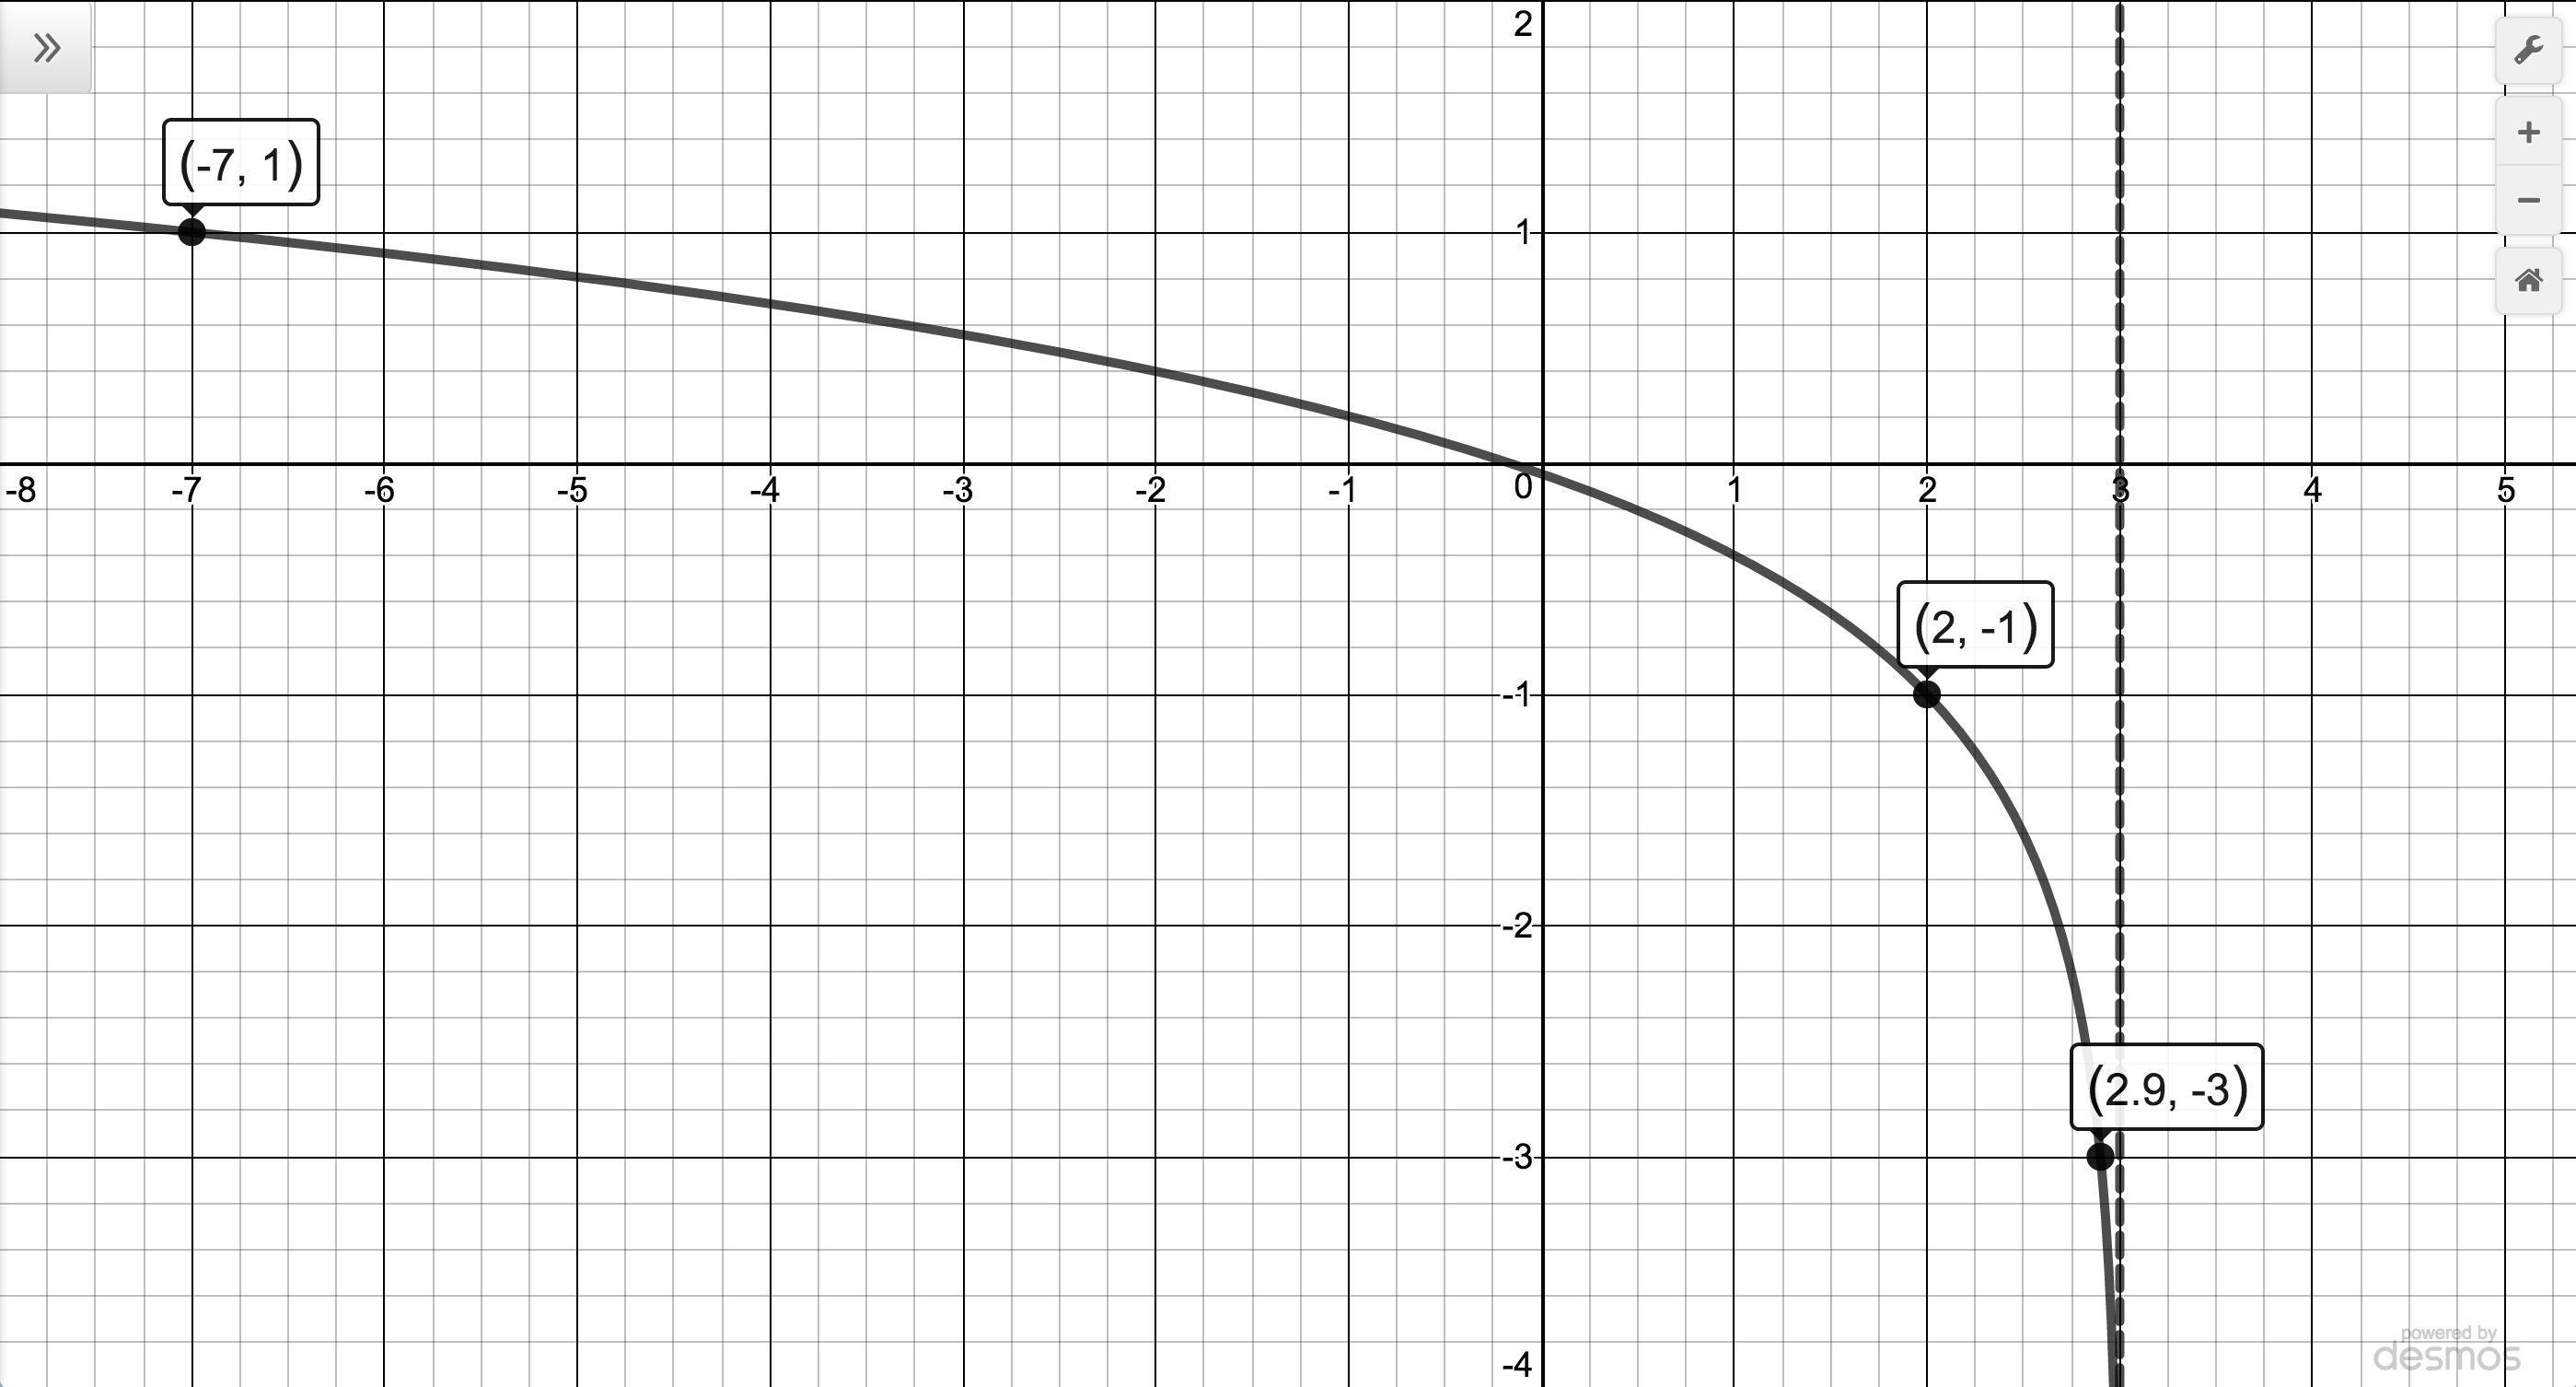
\includegraphics[height=2in]{./LogarithmicFunctionsGraphics/LogarithmicFunctionsEx01a.jpg}}

Note that in this case, we can graph $f$ using transformations, which we do so here for extra practice. 

\smallskip


Taking a cue from Theorem \ref{transformationsthm}, we rewrite $f(x) = 2 \log_{10}(-x+3) -1$ and  view this function as a transformed version of $h(x) = \log_{10}(x)$. 



\smallskip

To graph $y = \log(x) = \log_{10}(x)$,  We select three points to track corresponding to powers of $10$:  $(0.1, -1)$, $(1,0)$ and $(10,1)$, along with the vertical asymptote $x=0$.   


\smallskip

Since $f(x) = 2h(-x+3)-1$, Theorem \ref{transformationsthm} tells us that to obtain the destinations of these points, we first subtract $3$ from the $x$-coordinates (shifting the graph left $3$ units), then divide (multiply) by the $x$-coordinates by $-1$ (causing a reflection across the $y$-axis).   


\smallskip

Next, we multiply the $y$-coordinates by $2$ which results in a vertical stretch by a factor of $2$, then we finish by subtracting $1$ from the $y$-coordinates which shifts the graph down $1$ unit.  


\smallskip

Tracking points, we find:   $(0.1, -1) \rightarrow  (-2.9, -1) \rightarrow (2.9, -1) \rightarrow (2.9, -2) \rightarrow (2.9, -3)$, $(1,0) \rightarrow (-2,0) \rightarrow (2,0) \rightarrow (2,0) \rightarrow (2,-1)$, and  $(10,1) \rightarrow (7,1) \rightarrow (-7,1) \rightarrow (-7,2) \rightarrow (-7,1)$.  The vertical shift and reflection about the $y$-axis affects the vertical asymptote:  $x = 0 \rightarrow x = -3 \rightarrow x = 3$.  


\smallskip

Plotting these three points along with the vertical asymptote produces the graph of $f$ as seen above.


\item  To find the domain of $g$, we need to solve the inequality $\frac{x}{x-1} > 0$ using a sign diagram.\footnote{See Section \ref{RationalGraphs} for a review of this process, if needed.}  

\smallskip

If we define $r(x) = \frac{x}{x-1}$, we find $r$ is undefined at $x=1$ and $r(x) = 0$ when $x=0$.  Choosing some test values, we generate the sign diagram below on the left.  

\smallskip

We find $ \frac{x}{x-1} > 0$ on $(-\infty, 0) \cup (1, \infty)$ which is the domain of  $g$. The graph below confirms this.


\begin{center}

\begin{multicols}{2}

\begin{mfpic}[10]{-5}{5}{-1}{2}
\arrow \reverse \arrow \polyline{(-5,0),(5,0)}
\xmarks{-2,2}
\tlabel[cc](-3.5,1){$(+)$}
\tlabel[cc](-2,-1){$0$}
\tlabel[cc](-2,1){$0$}
\tlabel[cc](0,1){$(-)$}
\tlabel[cc](2,-1){$1$}
\tlabel[cc](2,1){\textinterrobang}
\tlabel[cc](3.5,1){$(+)$}
\end{mfpic}

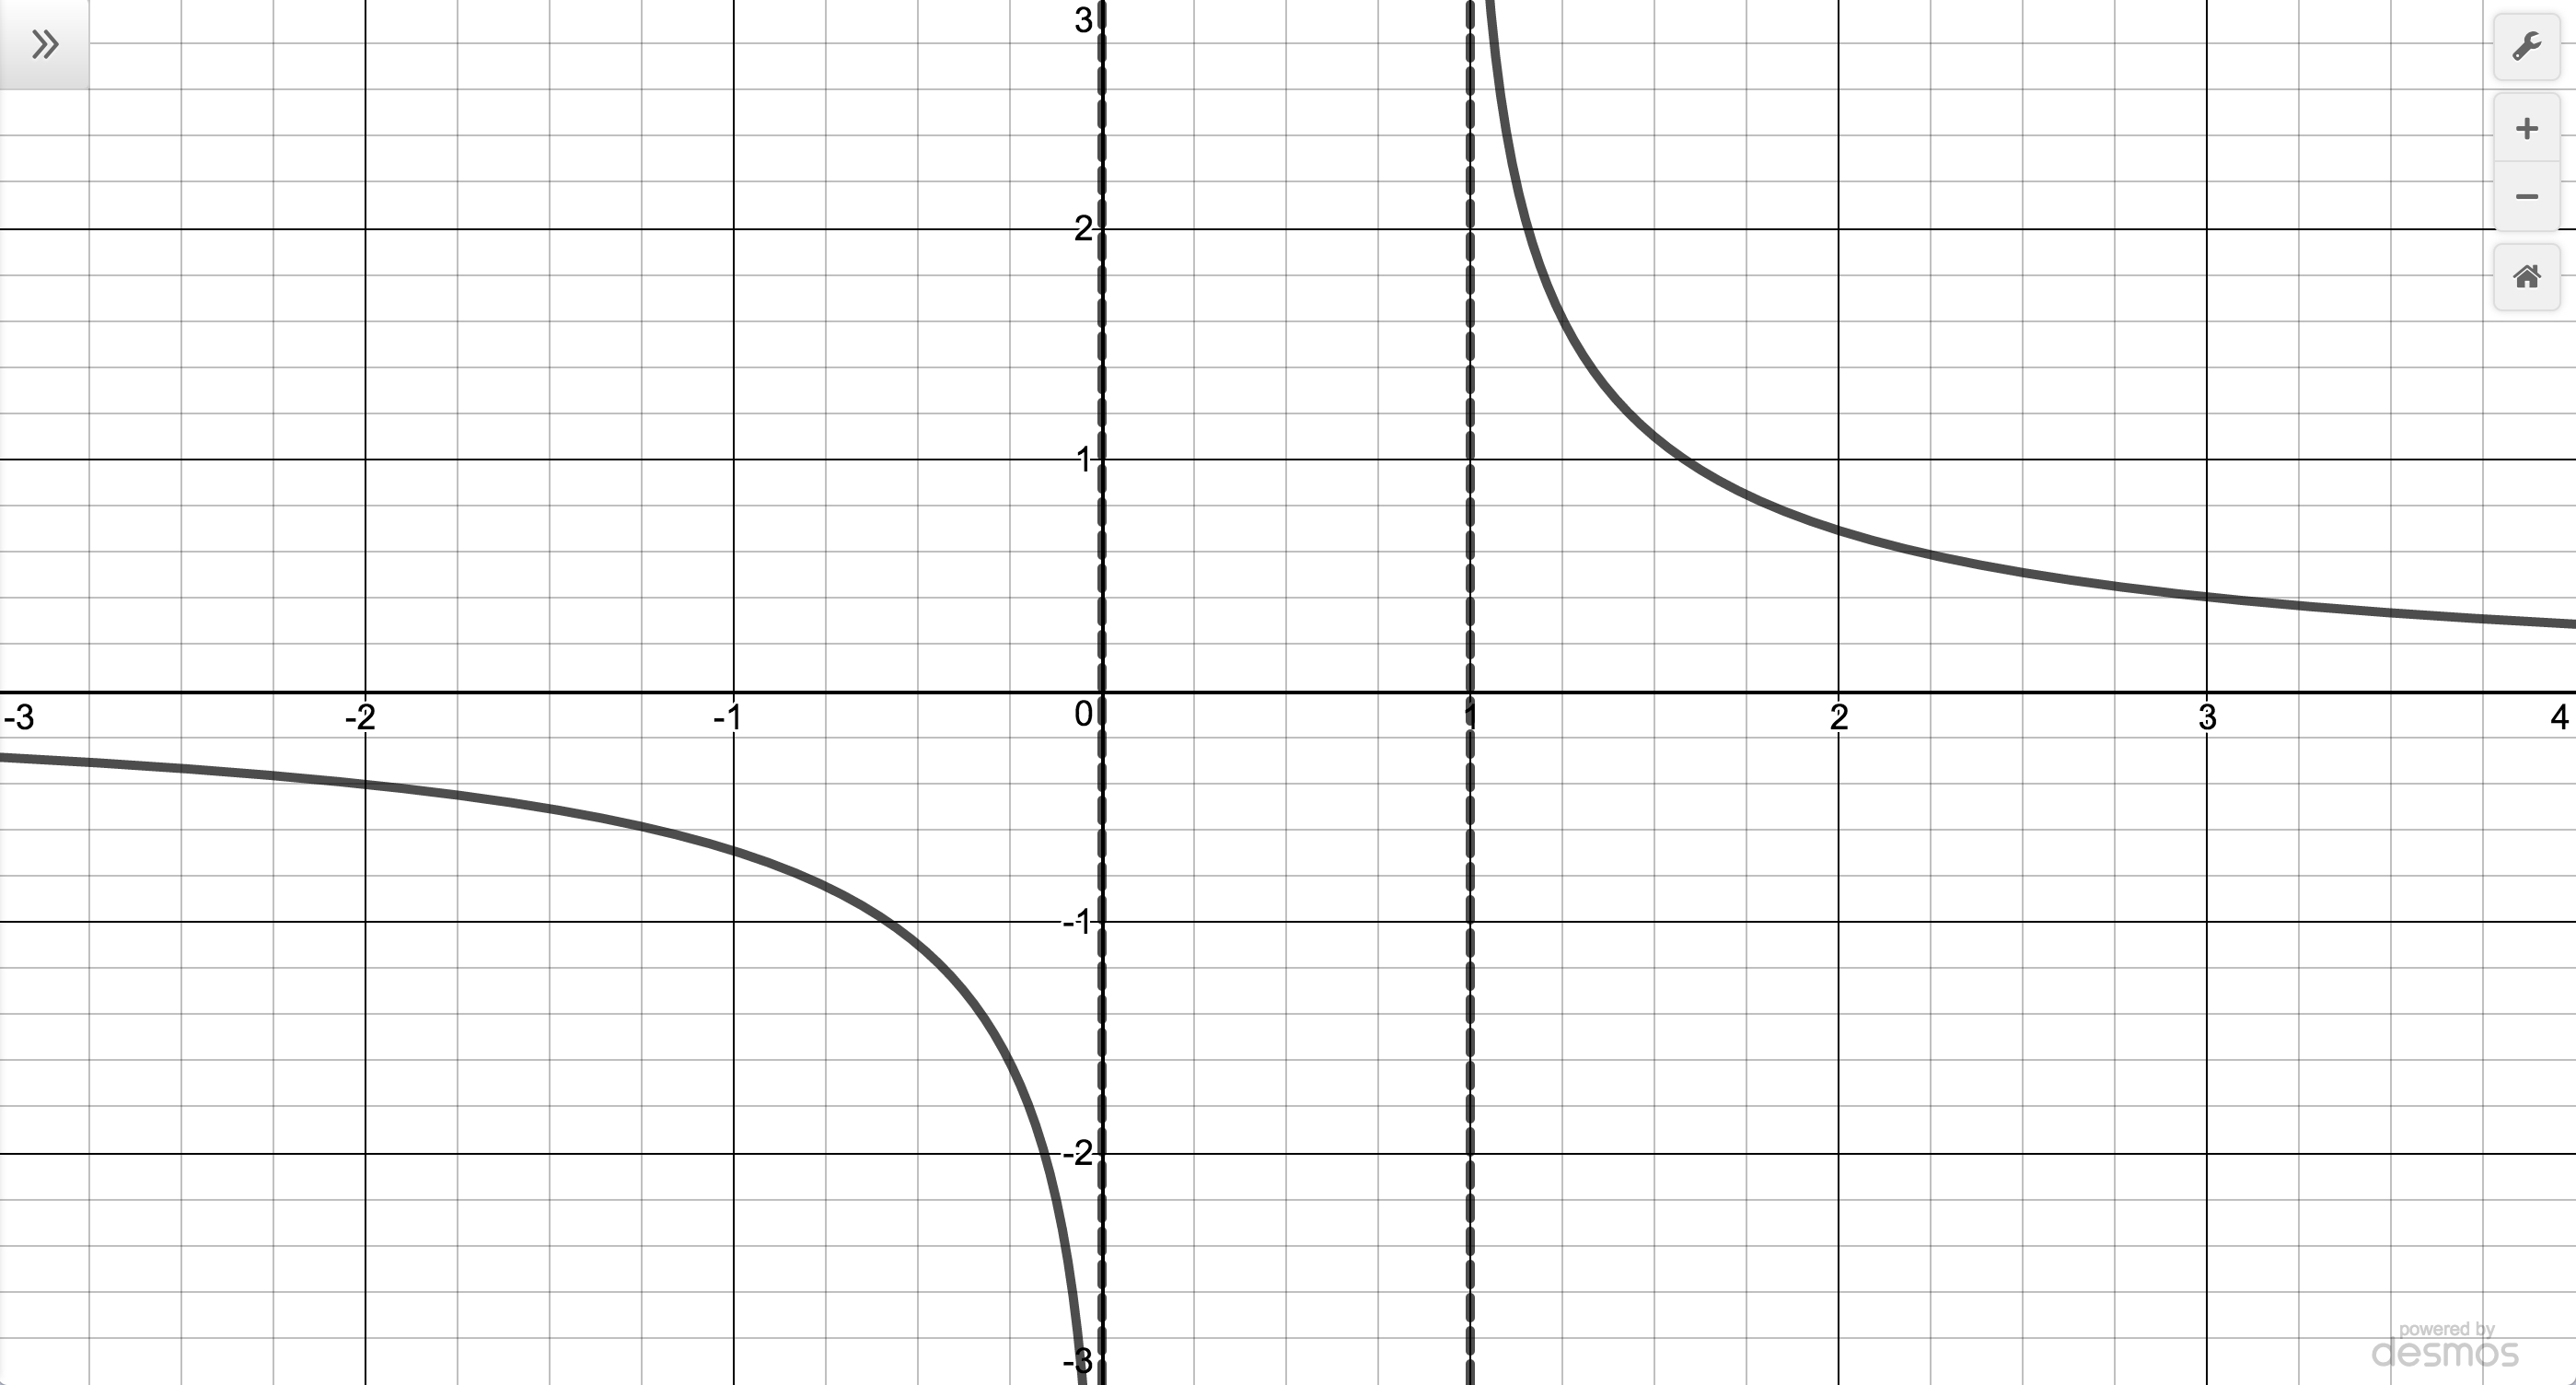
\includegraphics[width=3in]{./LogarithmicFunctionsGraphics/LogarithmicFunctionsEx01b.jpg}

\end{multicols}

\end{center}

  We can tell from the graph of $g$ that it is not the result of Section \ref{Transformations} transformations being applied to the graph $y = \ln(x)$, (do you see why?)  so barring a more detailed analysis using Calculus, producing a graph using a graphing utility is the best we can do.  
  
  \smallskip

One thing worthy of note, however, is the end behavior of $g$.  The graph suggests that as $x \rightarrow \pm \infty$, $g(x) \rightarrow 0$.  We can verify this analytically.  Using results  from Chapter \ref{RationalFunctions} and continuity, we know that as $x \rightarrow \pm \infty$, $\frac{x}{x-1} \approx 1$.  Hence, it makes sense that $g(x) = \ln \left(\frac{x}{x-1}\right) \approx \ln(1) = 0$.  \qed

\end{enumerate}

\end{ex}

While logarithms have some interesting applications of their own which you'll explore in the exercises, their primary use to us will be to undo exponential functions. (This is, after all, how they were defined.)  Our last example  reviews not only the major topics of this section, but reviews the salient points from Section \ref{InverseFunctions}.

\newpage

\begin{ex}  Let $f(x) = 2^{x-1} - 3$. \label{proceduralinverse}

\begin{enumerate}

\item  Graph $f$ using transformations and state the domain and range of $f$.

\item  Explain why $f$ is invertible and find a formula for $f^{-1}(x)$.

\item  Graph $f^{-1}$ using transformations and state the domain and range of $f^{-1}$.

\item  Verify $\left(f^{-1} \circ f\right)(x) = x$ for all $x$ in the domain of $f$ and  $\left(f \circ f^{-1} \right)(x) = x$ for all $x$ in the domain of $f^{-1}$.

\item  Graph $f$ and $f^{-1}$ on the same set of axes and check for symmetry about the line $y = x$.

\item  Use $f$ or $f^{-1}$ to solve the following equations.  Check your answers algebraically.

\begin{multicols}{2}

\begin{enumerate}

\item  $2^{x-1} - 3 = 4$

\item  $\log_{2}(t+3)+1 = 0$

\end{enumerate}

\end{multicols}

\end{enumerate}

{\bf Solution.}  

\begin{enumerate}

\item   To graph $f(x) = 2^{x-1} - 3$ using  Theorem \ref{transformationsthm}, we first identify $g(x) = 2^{x}$ and note  $f(x) = g(x-1)-3$.  Choosing the `control points' of  $\left(-1, \frac{1}{2}\right)$, $(0,1)$ and $(1, 2)$ on the graph of $g$ along with the horizontal asymptote $y=0$, we implement the algorithm set forth in Theorem \ref{transformationsthm}.  

\smallskip

First, we first add $1$ to the $x$-coordinates of the points on the graph of $g$ which shifts the the graph of $g$ to the right one unit.   Next, we subtract $3$ from each of the $y$-coordinates on this new graph, shifting the graph down $3$ units to get the graph of $f$.

\smallskip

Looking point-by-point, we have  $\left(-1, \frac{1}{2}\right) \rightarrow \left(0, \frac{1}{2}\right) \rightarrow \left(0, -\frac{5}{2}\right)$,  $(0,1)  \rightarrow (1,1)  \rightarrow  (1,-2)$, and, finally, $(1, 2) \rightarrow (2, 2) \rightarrow (2, -1)$.  The horizontal asymptote is affected only by the vertical shift, $y = 0 \rightarrow y = -3$.  

\smallskip

From the graph of $f$, we get the domain is $(-\infty, \infty)$ and the range is $(-3, \infty)$.


\[\begin{array}{ccc}

\begin{mfpic}[15]{-4}{5}{-3.25}{8.25}
\axes
\tlabel[cc](5,-0.5){\scriptsize $x$}
\tlabel[cc](0.5,8.25){\scriptsize $y$}
\tcaption{\scriptsize $y = h(x) = 2^{x}$}
\xmarks{-3,-2,-1,1,2,3,4}
\ymarks{-3,-2,-1,1,2,3,4,5,6,7}
\tlpointsep{4pt}
\axislabels {x}{{\scriptsize $-3 \hspace{7pt}$} -3, {\scriptsize $-2 \hspace{7pt}$} -2, {\scriptsize $-1 \hspace{7pt}$} -1, {\scriptsize $1$} 1, {\scriptsize $2$} 2, {\scriptsize $3$} 3, {\scriptsize $4$} 4}
\axislabels {y}{{\scriptsize $-3$} -3, {\scriptsize $-2$} -2, {\scriptsize $-1$} -1,{\scriptsize $1$} 1, {\scriptsize $2$} 2, {\scriptsize $3$} 3, {\scriptsize $4$} 4, {\scriptsize $5$} 5, {\scriptsize $6$} 6, {\scriptsize $7$} 7}
\penwd{1.25pt}
\arrow \reverse \arrow \function{-3.5, 3, 0.1}{2**x}
\point[4pt]{(-1,0.5), (0,1), (1,2)}
\end{mfpic}

&

\xrightarrow{\hspace{1in}}

&

\begin{mfpic}[15]{-4}{5}{-3.25}{8.25}
\axes
\dashed \polyline{(-4,-3),(5,-3)}
\tlabel[cc](5,-0.5){\scriptsize $x$}
\tlabel[cc](0.5,8.25){\scriptsize $y$}
\tcaption{\scriptsize $y = f(x) = 2^{x-1}-3$}
\xmarks{-3,-2,-1,1,2,3,4}
\ymarks{-3,-2,-1,1,2,3,4,5,6,7}
\tlpointsep{4pt}
\axislabels {x}{{\scriptsize $-3 \hspace{7pt}$} -3, {\scriptsize $-2 \hspace{7pt}$} -2, {\scriptsize $-1 \hspace{7pt}$} -1, {\scriptsize $1$} 1, {\scriptsize $2$} 2, {\scriptsize $3$} 3, {\scriptsize $4$} 4}
\axislabels {y}{{\scriptsize $-2$} -2, {\scriptsize $-1$} -1,{\scriptsize $1$} 1, {\scriptsize $2$} 2, {\scriptsize $3$} 3, {\scriptsize $4$} 4, {\scriptsize $5$} 5, {\scriptsize $6$} 6, {\scriptsize $7$} 7}
\penwd{1.25pt}
\arrow \reverse \arrow \function{-2.5, 4, 0.1}{(2**(x-1))-3}
\point[4pt]{(0,-2.5), (1,-2), (2,-1)}
\end{mfpic} \\

\end{array}\]

\item  The graph of $f$ passes the Horizontal Line Test so $f$ is one-to-one, hence invertible.  

\smallskip

To find a formula for $f^{-1}(x)$, we normally set $y=f(x)$, interchange the $x$ and $y$, then proceed to solve for $y$.  Doing so in this situation leads us to the equation $x = 2^{y-1}-3$.  We have yet to discuss how to solve this kind of equation, so we will attempt to find the formula for $f^{-1}$ procedurally.  

\smallskip

Thinking of $f$ as a process, the formula $f(x) = 2^{x-1}-3$ takes an input $x$ and applies the steps: first subtract $1$.   Second put the result of the first step as the exponent on $2$.   Last, subtract $3$ from the result of the second step.

\smallskip

Clearly, to undo subtracting $1$, we will add $1$, and similarly we undo subtracting $3$ by adding $3$.  How do we undo the second step?  The answer is we use the logarithm.  

\smallskip

By definition, $\log_{2}(x)$ undoes exponentiation by $2$.  Hence, $f^{-1}$ should: first,  add $3$.  Second,  take the logarithm base $2$ of the result of the first step. Lastly,  add $1$ to the result of the second ste.  In symbols, $f^{-1}(x) = \log_{2}(x+3)+1$.  


\item  To graph $f^{-1}(x) = \log_{2}(x+3)+1$ using Theorem \ref{transformationsthm}, we start with $j(x) = \log_{2}(x)$ and track the points $\left(\frac{1}{2},-1\right)$, $(1,0)$ and $(2, 1)$ on the graph of $j$ along with the vertical asymptote $x=0$ through the transformations.

\smallskip

Since $f^{-1}(x) = j(x+3)+1$, we first subtract $3$ from each of the $x$-coordinates of each of the points on the graph of $y=j(x)$ shifting the graph of $j$ to the left three units.  We then add $1$ to each of the $y$-coordinates of the points on this new graph, shifting the graph up one unit. 

\smallskip

Tracking points, we get   $\left(\frac{1}{2},-1\right) \rightarrow \left(-\frac{5}{2},-1\right) \rightarrow \left(-\frac{5}{2},0\right)$, $(1,0) \rightarrow (-2,1) \rightarrow (-2,2)$, and $(2, 1) \rightarrow (-1, 1) \rightarrow (-1, 2)$.  

\smallskip

The vertical asymptote is only affected by the horizontal shift, so we have $x = 0 \rightarrow x = -3$.

\smallskip

From the graph below, we  get the  domain of $f^{-1}$ is $(-3, \infty)$, which matches the range of $f$, and the range of $f^{-1}$ is $(-\infty, \infty)$, which matches the domain of $f$, in accordance with Theorem \ref{inversefunctionprops}.

\[\begin{array}{ccc}

\begin{mfpic}[15]{-4}{9}{-4}{5}

\axes
\tlabel[cc](9,-0.5){\scriptsize $x$}
\tlabel[cc](0.5,5){\scriptsize $y$}
\tcaption{\scriptsize $y = j(x) = \log_{2}(x)$}
\ymarks{-3,-2,-1,1,2,3,4}
\xmarks{-3,-2,-1,1,2,3,4,5,6,7,8}
\tlpointsep{4pt}
\axislabels {y}{{\scriptsize $-3$} -3,{\scriptsize $-2$} -2, {\scriptsize $-1$} -1, {\scriptsize $1$} 1, {\scriptsize $2$} 2, {\scriptsize $3$} 3, {\scriptsize $4$} 4}
\axislabels {x}{{\scriptsize $-3 \hspace{7pt}$} -3, {\scriptsize $-2 \hspace{7pt}$} -2, {\scriptsize $-1 \hspace{7pt}$} -1,{\scriptsize $1$} 1, {\scriptsize $2$} 2, {\scriptsize $3$} 3, {\scriptsize $4$} 4, {\scriptsize $5$} 5, {\scriptsize $6$} 6, {\scriptsize $7$} 7, {\scriptsize $8$} 8}
\penwd{1.25pt}
\arrow \reverse \arrow \parafcn{-3.5, 3.1, 0.1}{(2**t,t)}
\point[4pt]{(0.5,-1), (1,0), (2,1)}
\end{mfpic}

&

\xrightarrow{\hspace{1in}}

&

\begin{mfpic}[15]{-4}{9}{-4}{5}
\axes
\tlabel[cc](9,-0.5){\scriptsize $x$}
\tlabel[cc](0.5,5){\scriptsize $y$}
\tcaption{\scriptsize $y = f^{-1}(x) = \log_{2}(x+3)+1$}
\ymarks{-3,-2,-1,1,2,3,4}
\xmarks{-3,-2,-1,1,2,3,4,5,6,7,8}
\tlpointsep{4pt}
\axislabels {y}{{\scriptsize $-3$} -3,{\scriptsize $-2$} -2, {\scriptsize $-1$} -1, {\scriptsize $1$} 1, {\scriptsize $2$} 2, {\scriptsize $3$} 3, {\scriptsize $4$} 4}
\axislabels {x}{{\scriptsize $-2 \hspace{7pt}$} -2, {\scriptsize $-1 \hspace{7pt}$} -1,{\scriptsize $1$} 1, {\scriptsize $2$} 2, {\scriptsize $3$} 3, {\scriptsize $4$} 4, {\scriptsize $5$} 5, {\scriptsize $6$} 6, {\scriptsize $7$} 7, {\scriptsize $8$} 8}
\dashed \polyline{(-3,-4),(-3,5)}
\penwd{1.25pt}
\point[4pt]{(-2.5,0), (-2,1), (-1,2)}
\arrow \reverse \arrow \parafcn{-2.5, 4.1, 0.1}{((2**(t-1))-3,t)}
\end{mfpic} \\

\end{array}\]

\item  We now verify that $f(x) = 2^{x-1}-3$ and $f^{-1}(x) = \log_{2}(x+3)+1$ satisfy the composition requirement for inverses.  When simplifying $(f^{-1} \circ f)(x)$ we assume $x$ can be any real number while when simplifying $(f \circ f^{-1})(x)$, we restrict our attention to $x > -3$. (Do you see why?)  

\smallskip

Note the use of the inverse properties of exponential and logarithmic functions  from Theorem \ref{logfcnprops} when it comes to simplifying expressions of the form $\log_{2}(2^{u})$ and $2^{\log_{2}(u)}$. 

\begin{multicols}{2}


$\begin{array}{rcl}

\left(f^{-1}\circ f\right)(x) & = & f^{-1}(f(x))  \\

& = & f^{-1}\left(2^{x-1}-3 \right)  \\

& = & \log_{2}\left( \left[2^{x-1}-3\right]+3 \right)+1  \\

& = & \log_{2}\left( 2^{x-1} \right)+1  \\

& = & (x-1) +1  \\

& = & x \, \, \checkmark \\

\end{array}$



$\begin{array}{rcl}

\left(f\circ f^{-1}\right)(x) & = & f\left(f^{-1}(x)\right) \\

& = & f\left( \log_{2}(x+3)+1 \right) \\

& = & 2^{\left( \log_{2}(x+3)+1 \right)-1} - 3 \\

& = & 2^{\log_{2}(x+3)} - 3  \\

& = & (x+3) -3  \\

& = & x \, \, \checkmark \\

\end{array}$

\end{multicols}


\item  Last, but certainly not least, we graph $y=f(x)$ and $y=f^{-1}(x)$ on the same set of axes and observe the symmetry about the line $y=x$.

\begin{center}
\begin{mfpic}[15]{-4}{7}{-4}{7}
\axes
\tlabel[cc](7,-0.5){\scriptsize $x$}
\tlabel[cc](0.5,7){\scriptsize $y$}
\tlabel(-4,-5){\scriptsize $y = f(x) = 2^{x-1}-3$}
\tlabel(-4,-6){\text{\scriptsize  \boldmath $y = f^{-1}(x) = \log_{2}(x+3)+1$}}
\xmarks{-3,-2,-1,1,2,3,4,5,6}
\ymarks{-3,-2,-1,1,2,3,4,5,6}
\tlpointsep{4pt}
\axislabels {x}{{\scriptsize $-3 \hspace{7pt}$} -3, {\scriptsize $-2 \hspace{7pt}$} -2, {\scriptsize $-1 \hspace{7pt}$} -1, {\scriptsize $1$} 1, {\scriptsize $2$} 2, {\scriptsize $3$} 3, {\scriptsize $4$} 4, {\scriptsize $5$} 5, {\scriptsize $6$} 6}
\axislabels {y}{{\scriptsize $-2$} -2, {\scriptsize $-1$} -1,{\scriptsize $1$} 1, {\scriptsize $2$} 2, {\scriptsize $3$} 3, {\scriptsize $4$} 4, {\scriptsize $5$} 5, {\scriptsize $6$} 6}
\arrow \reverse \arrow \function{-4.1, 4.1, 0.1}{(2**(x-1))-3}
\dashed \polyline{(-4,-3),(5,-3)}
\dashed \polyline{(-3,-3),(6,6)}
\dashed \polyline{(-3,-4),(-3,5)}
\penwd{1.5pt}
\arrow \reverse \arrow \parafcn{-4.1, 4.1, 0.1}{((2**(t-1))-3,t)}
\end{mfpic}

\end{center}
\end{enumerate}

\item  \begin{enumerate}

\item  Viewing $2^{x-1} - 3 = 4$ as $f(x) = 4$, we apply $f^{-1}$ to `undo' $f$ to get $f^{-1}(f(x)) = f^{-1}(4)$, which reduces to $x = f^{-1}(4)$.  Since we have shown (algebraically and graphically!) that $f^{-1}(x) =  \log_{2}(x+3) + 1$, we get  $x = f^{-1}(4) = \log_{2}(4+3) + 1 = \log_{2}(7) + 1$. 

\smallskip

Alternatively, we know from Theorem \ref{inversefunctionprops} that $f(x) = 4$ is equivalent to $x = f^{-1}(4)$ directly.

\smallskip


Note  that since, by definition,  $2^{\log_{2}(7)} = 7$,  $2^{( \log_{2}(7) + 1)-1} - 3 = 2^{\log_{2}(7)} - 3  = 7 - 3 = 4$, as required.

\item  Since we may think of the equation $\log_{2}(t+3)+1 = 0$ as $f^{-1}(t) = 0$, we can solve this equation by applying $f$ to both sides to get $f(f^{-1}(t)) = f(0)$ or $t = 2^{0-1} -3 = \frac{1}{2} - 3 = -\frac{5}{2}$.

Since $\log_{2}(2^{-1}) = -1$, we get  $\log_{2}\left(-\frac{5}{2} +3 \right)+1 = \log_{2}\left( \frac{1}{2} \right) + 1 =  \log_{2}(2^{-1})-1 + 1 = 0$, as required. \qed

\end{enumerate}

\end{ex}

\newpage

\subsection{Exercises}

\label{ExercisesforLogarithmicFunctions}

\label{IntroExpLogsExercises}

In Exercises \ref{rewritefirstex} - \ref{rewritelastex}, use the property: $b^{a} = c$ if and only if $\log_{b}(c) = a$ from Theorem \ref{logfcnprops} to rewrite the given equation in the other form.  That is, rewrite the exponential equations as logarithmic equations and rewrite the logarithmic equations as exponential equations.

\begin{multicols}{3}
\begin{enumerate}

\item  $2^{3} = 8$ \label{rewritefirstex}

\item  $5^{-3} = \frac{1}{125}$  

\item  $4^{5/2} = 32$  

\setcounter{HW}{\value{enumi}}
\end{enumerate}
\end{multicols}

\begin{multicols}{3}
\begin{enumerate}
\setcounter{enumi}{\value{HW}}

\item  $\left(\frac{1}{3}\right)^{-2} = 9$  

\item  $\left(\frac{4}{25}\right)^{-1/2} = \frac{5}{2}$  

\item  $10^{-3} = 0.001$ 

\setcounter{HW}{\value{enumi}}
\end{enumerate}
\end{multicols}

\begin{multicols}{3}
\begin{enumerate}
\setcounter{enumi}{\value{HW}}

\item  $e^{0}  = 1$  

\item  $\log_{5}(25) = 2$  

\item  $\log_{25} (5) = \frac{1}{2}$  

\setcounter{HW}{\value{enumi}}
\end{enumerate}
\end{multicols}

\begin{multicols}{3}
\begin{enumerate}
\setcounter{enumi}{\value{HW}}

\item  $\log_{3} \left(\frac{1}{81} \right) = -4$  

\item  $\log_{\frac{4}{3}} \left(\frac{3}{4} \right) = -1$  

\item  $\log(100) = 2$  

\setcounter{HW}{\value{enumi}}
\end{enumerate}
\end{multicols}

\begin{multicols}{3}
\begin{enumerate}
\setcounter{enumi}{\value{HW}}

\item  $\log (0.1) = -1$  

\item  $\ln(e) = 1$ 

\item  $\ln\left(\frac{1}{\sqrt{e}}\right) = -\frac{1}{2}$  \label{rewritelastex}

\setcounter{HW}{\value{enumi}}
\end{enumerate}
\end{multicols}

In Exercises \ref{simplifylogfirst} - \ref{simplifyloglast}, evaluate the expression without using a calculator.

\begin{multicols}{3}
\begin{enumerate}
\setcounter{enumi}{\value{HW}}

\item $\log_{3} (27)$  \label{simplifylogfirst}
\item $\log_{6} (216)$
\item $\log_{2} (32)$

\setcounter{HW}{\value{enumi}}
\end{enumerate}
\end{multicols}


\begin{multicols}{3}
\begin{enumerate}
\setcounter{enumi}{\value{HW}}

\item  $\log_{6} \left( \frac{1}{36} \right)$
\item $\log_{8} (4)$
\item $\log_{36} (216)$

\setcounter{HW}{\value{enumi}}
\end{enumerate}
\end{multicols}


\begin{multicols}{3}
\begin{enumerate}
\setcounter{enumi}{\value{HW}}

\item $\log_{\frac{1}{5}} (625)$
\item  $\log_{\frac{1}{6}} (216)$
\item $\log_{36} (36)$ 

\setcounter{HW}{\value{enumi}}
\end{enumerate}
\end{multicols}


\begin{multicols}{3}
\begin{enumerate}
\setcounter{enumi}{\value{HW}}

\item $\log \left(\frac{1}{1000000}\right)$
\item $\log(0.01)$
\item $\ln\left(e^3\right)$

\setcounter{HW}{\value{enumi}}
\end{enumerate}
\end{multicols}


\begin{multicols}{3}
\begin{enumerate}
\setcounter{enumi}{\value{HW}}

\item $\log_{4} (8)$
\item $\log_{6} (1)$
\item $\log_{13} \left(\sqrt{13}\right)$

\setcounter{HW}{\value{enumi}}
\end{enumerate}
\end{multicols}


\begin{multicols}{3}
\begin{enumerate}
\setcounter{enumi}{\value{HW}}

\item $\log_{36} \left(\sqrt[4]{36}\right)$
\item $7^{\log_{7} (3)}$
\item  $36^{\log_{36}(216)}$

\setcounter{HW}{\value{enumi}}
\end{enumerate}
\end{multicols}


\begin{multicols}{3}
\begin{enumerate}
\setcounter{enumi}{\value{HW}}

\item  $\log_{36} \left(36^{216}\right)$
\item $\ln \left(e^{5} \right)$
\item $\log \left(\sqrt[9]{10^{11}}\right)$

\setcounter{HW}{\value{enumi}}
\end{enumerate}
\end{multicols}


\begin{multicols}{3}
\begin{enumerate}
\setcounter{enumi}{\value{HW}}

\item  $\log\left( \sqrt[3]{10^5} \right)$
\item  $\ln \left( \frac{1}{\sqrt{e}}\right)$
\item $\log_{5} \left(3^{\log_{3} (5)}\right)$

\setcounter{HW}{\value{enumi}}
\end{enumerate}
\end{multicols}


\begin{multicols}{3}
\begin{enumerate}
\setcounter{enumi}{\value{HW}}

\item $\log\left(e^{\ln(100)}\right)$ 
\item $\log_{2}\left(3^{-\log_{3}(2)}\right)$
\item $\ln\left(42^{6\log(1)}\right)$ \label{simplifyloglast}

\setcounter{HW}{\value{enumi}}
\end{enumerate}
\end{multicols}

In Exercises \ref{domainlogfirst} - \ref{domainloglast}, find the domain of the function.

\begin{multicols}{2}
\begin{enumerate}
\setcounter{enumi}{\value{HW}}


\item $f(x) = \ln(x^{2} + 1)$ \label{domainlogfirst}
\item $f(x) = \log_{7}(4x + 8)$

\setcounter{HW}{\value{enumi}}
\end{enumerate}
\end{multicols}

\begin{multicols}{2}
\begin{enumerate}
\setcounter{enumi}{\value{HW}}


\item $g(t) = \ln(4t-20)$
\item $g(t) = \log \left(t^2+9t+18\right)$

\setcounter{HW}{\value{enumi}}
\end{enumerate}
\end{multicols}

\begin{multicols}{2}
\begin{enumerate}
\setcounter{enumi}{\value{HW}}

\item $f(x) = \log \left(\dfrac{x + 2}{x^{2} - 1}\right)$
\item $f(x) = \log\left(\dfrac{x^2+9x+18}{4x-20}\right)$

\setcounter{HW}{\value{enumi}}
\end{enumerate}
\end{multicols}

\begin{multicols}{2}
\begin{enumerate}
\setcounter{enumi}{\value{HW}}

\item $g(t) = \ln(7 - t) + \ln(t - 4)$
\item $g(t) = \ln(4t-20) + \ln\left(t^2+9t+18\right)$

\setcounter{HW}{\value{enumi}}
\end{enumerate}
\end{multicols}

\begin{multicols}{2}
\begin{enumerate}
\setcounter{enumi}{\value{HW}}

\item $f(x) = \log\left(x^2+x+1\right)$
\item $f(x) = \sqrt[4]{\log_{4} (x)}$

\setcounter{HW}{\value{enumi}}
\end{enumerate}
\end{multicols}

\begin{multicols}{2}
\begin{enumerate}
\setcounter{enumi}{\value{HW}}

\item $g(t) = \log_{9}(|t + 3| - 4)$
\item $g(t) = \ln(\sqrt{t - 4} - 3)$

\setcounter{HW}{\value{enumi}}
\end{enumerate}
\end{multicols}

\begin{multicols}{2}
\begin{enumerate}
\setcounter{enumi}{\value{HW}}

\item $f(x) = \dfrac{1}{3 - \log_{5} (x)}$
\item $f(x) = \dfrac{\sqrt{-1 - x}}{\log_{\frac{1}{2}} (x)}$

\setcounter{HW}{\value{enumi}}
\end{enumerate}
\end{multicols}

\begin{multicols}{2}
\begin{enumerate}
\setcounter{enumi}{\value{HW}}

\item $f(x) = \ln(-2x^{3} - x^{2} + 13x - 6)$  \label{domainloglast}

\setcounter{HW}{\value{enumi}}
\end{enumerate}
\end{multicols}


In Exercises \ref{graphlogfirst} - \ref{graphloglast}, sketch the graph of $y=g(x)$ by starting with the graph of $y = f(x)$ and using transformations.  Track at least three points of your choice and the vertical asymptote through the transformations. State the domain and range of $g$.


\begin{multicols}{2}
\begin{enumerate}
\setcounter{enumi}{\value{HW}}

\item  $f(x) = \log_{2}(x)$, $g(x) = \log_{2}(x+1)$ \label{graphlogfirst}

\item  $f(x) = \log_{\frac{1}{3}}(x)$, $g(x) = \log_{\frac{1}{3}}(x)+1$

\setcounter{HW}{\value{enumi}}
\end{enumerate}
\end{multicols}

\begin{multicols}{2}
\begin{enumerate}
\setcounter{enumi}{\value{HW}}


\item  $f(x) = \log_{3}(x)$, $g(x) = -\log_{3}(x-2)$

\item  $f(x) = \log(x)$, $g(x) = 2\log(x+20) -1$  

\setcounter{HW}{\value{enumi}}
\end{enumerate}
\end{multicols}

\begin{multicols}{2}
\begin{enumerate}
\setcounter{enumi}{\value{HW}}

\item  $g(t) = \log_{0.5}(t)$, $g(t) = 10 \log_{0.5}\left(\frac{t}{100}\right)$

\item  $g(t) = \log_{1.25}(t)$, $g(t) = \log_{1.25}(-t+1) + 2$

\setcounter{HW}{\value{enumi}}
\end{enumerate}
\end{multicols}

\begin{multicols}{2}
\begin{enumerate}
\setcounter{enumi}{\value{HW}}


\item  $g(t) = \ln(t)$, $g(t) = -\ln(8-t)$

\item  $g(t) = \ln(t)$, $g(t) = -10\ln\left(\frac{t}{10}\right)$ \label{graphloglast}

\setcounter{HW}{\value{enumi}}
\end{enumerate}
\end{multicols}

\begin{enumerate}
\setcounter{enumi}{\value{HW}}

\smallskip

\item  Verify that each function in Exercises \ref{graphlogfirst} - \ref{graphloglast} is the inverse of the corresponding function in Exercises \ref{graphexpfirsta} - \ref{graphexplasta} in Section \ref{ExponentialFunctions}.  (Match up \#\ref{graphexpfirsta} and \#\ref{graphlogfirst}, and so on.)

\setcounter{HW}{\value{enumi}}
\end{enumerate}

In Exercises, \ref{logformfirsta} - \ref{logformlasta}, the graph of a logarithmic function is given.  Find a formula for the function in the form $F(x) = a \cdot \log_{2}(bx-h)+k$.

\begin{multicols}{2}
\begin{enumerate}
\setcounter{enumi}{\value{HW}}

\item  \label{logformfirsta}  Points:  $\left( -\frac{5}{2}, -2 \right)$,  $\left(-2, -1 \right)$, $\left(-1,0 \right)$, \\
Asymptote:  $x = -3$. \\

\begin{mfpic}[13]{-4}{6}{-5}{3}
\axes
\tlabel[cc](6,-0.5){\scriptsize $x$}
\tlabel[cc](0.5,3){\scriptsize $y$}
\ymarks{-4, -3,-2,-1,1,2}
\xmarks{-3, -2, -1, 1,2,3,4,5}
\tlpointsep{4pt}
\axislabels {y}{{\scriptsize $-4$} -4,{\scriptsize $-3$} -3, {\scriptsize $-2$} -2, {\scriptsize $-1$} -1, {\scriptsize $1$} 1, {\scriptsize $2$} 2}
\axislabels {x}{{\scriptsize $1$} 1, {\scriptsize $2$} 2, {\scriptsize $3$} 3, {\scriptsize $4$} 4, {\scriptsize $5$} 5, {\scriptsize $-1 \hspace{7pt}$} -1, {\scriptsize $-2 \hspace{7pt}$} -2, {\scriptsize $-3 \hspace{7pt}$} -3}
\dashed \polyline{(-3,-5), (-3,3)}
\penwd{1.25pt}
\arrow \reverse \arrow \parafcn{-4.5, 2.1, 0.1}{( (2**(t+1))-3, t)}
\point[4pt]{(-2.5, -2), (-2,-1),(-1,0)}
\end{mfpic}

\vfill

\columnbreak

\item  Points:  $\left( 1, -1 \right)$, $\left( 2, 0 \right)$, $\left(\frac{5}{2}, 1 \right)$ \\
Asymptote:  $x = 3$. \\

\begin{mfpic}[13]{-6}{4}{-4}{4}
\axes
\tlabel[cc](4,-0.5){\scriptsize $x$}
\tlabel[cc](0.5,4){\scriptsize $y$}
\ymarks{-3,-2,-1,1,2,3}
\xmarks{-5 step 1 until 3}
\tlpointsep{4pt}
\axislabels {y}{{\scriptsize $-3$} -3, {\scriptsize $-2$} -2, {\scriptsize $-1$} -1, {\scriptsize $1$} 1, {\scriptsize $2$} 2, {\scriptsize $3$} 3}
\axislabels {x}{{\scriptsize $1$} 1, {\scriptsize $2$} 2, {\scriptsize $3$} 3, {\scriptsize $-1 \hspace{7pt}$} -1, {\scriptsize $-2 \hspace{7pt}$} -2, {\scriptsize $-3 \hspace{7pt}$} -3, {\scriptsize $-4 \hspace{7pt}$} -4, {\scriptsize $-5 \hspace{7pt}$} -5}
\dashed \polyline{(3,-4), (3,4)}
\penwd{1.25pt}
\arrow \reverse \arrow \parafcn{-3, 3.1, 0.1}{(3-(2**(-t)), t)}
\point[4pt]{(1,-1), (2,0), ( 2.5,1)}
\end{mfpic}


\setcounter{HW}{\value{enumi}}
\end{enumerate}
\end{multicols}

\begin{multicols}{2}
\begin{enumerate}
\setcounter{enumi}{\value{HW}}

\item  Points:  $\left(\frac{1}{2}, \frac{5}{2} \right)$, $\left(1, 3 \right)$, $\left(2, \frac{7}{2} \right)$, \\
Asymptote:  $x = 0$. \\

\begin{mfpic}[13]{-1}{9}{-1}{5}
\axes
\tlabel[cc](9,-0.5){\scriptsize $x$}
\tlabel[cc](0.5,5){\scriptsize $y$}
\ymarks{1 step 1 until 4}
\xmarks{1 step 1 until 8}
\tlpointsep{4pt}
\axislabels {y}{{\scriptsize $1$} 1, {\scriptsize $2$} 2, {\scriptsize $3$} 3, {\scriptsize $4$} 4}
\axislabels {x}{{\scriptsize $1$} 1, {\scriptsize $2$} 2, {\scriptsize $3$} 3, {\scriptsize $4$} 4, {\scriptsize $5$} 5, {\scriptsize $6$} 6, {\scriptsize $7$} 7, {\scriptsize $8$} 8}
\penwd{1.25pt}
\arrow \reverse \arrow \parafcn{1.25, 4.55, 0.1}{(2**(2*t-6), t)}
\point[4pt]{(0.5, 2.5), (1,3), (2,3.5) }
\end{mfpic}

\vfill

\columnbreak

\item  Points:  $\left( 6, -\frac{1}{2} \right)$, $\left(3,0 \right)$, $\left( \frac{3}{2}, \frac{1}{2} \right)$, \\
Asymptote:  $x = 0$.   \\

\begin{mfpic}[13]{-1}{9}{-4}{4}
\axes
\tlabel[cc](9,-0.5){\scriptsize $x$}
\tlabel[cc](0.5,4){\scriptsize $y$}
\ymarks{-3,-2,-1,1,2,3}
\xmarks{1,2,3,4,5,6,7,8}
\tlpointsep{4pt}
\axislabels {y}{{\scriptsize $-3$} -3, {\scriptsize $-2$} -2, {\scriptsize $-1$} -1, {\scriptsize $1$} 1, {\scriptsize $2$} 2, {\scriptsize $3$} 3}
\axislabels {x}{{\scriptsize $1$} 1, {\scriptsize $2$} 2, {\scriptsize $3$} 3,  {\scriptsize $7$} 7, {\scriptsize $8$} 8}
\penwd{1.25pt}
\arrow \reverse \arrow \parafcn{-0.79, 2, 0.1}{(3*(2**(-2*t)), t)}
\point[4pt]{(6, -0.5), (3,0), (1.5, 0.5)}
\end{mfpic}


\label{logformlasta} 

\setcounter{HW}{\value{enumi}}
\end{enumerate}
\end{multicols}


\begin{enumerate}
\setcounter{enumi}{\value{HW}}


\item \label{logformbase4exercise} Find a formula for each graph in Exercises \ref{logformfirsta} - \ref{logformlasta} of the form $G(x) =  a \cdot \log_{4}(bx-h)+k$.

\setcounter{HW}{\value{enumi}}
\end{enumerate}

In Exercises \ref{inverselogexpfirst} - \ref{inverselogexplast},  find the inverse of the function from the `procedural perspective' discussed in Example \ref{proceduralinverse} and graph the function and its inverse on the same set of axes.

\begin{multicols}{2}
\begin{enumerate}
\setcounter{enumi}{\value{HW}}

\item $f(x) = 3^{x + 2} - 4$  \label{inverselogexpfirst} 
\item $f(x) = \log_{4}(x - 1)$

\setcounter{HW}{\value{enumi}}
\end{enumerate}
\end{multicols}

\enlargethispage{.5in}
\vspace{-.2in}

\begin{multicols}{2}
\begin{enumerate}
\setcounter{enumi}{\value{HW}}

\item $g(t)= -2^{-t} + 1$
\item $g(t) = 5\log(t) - 2$ \label{inverselogexplast}

\setcounter{HW}{\value{enumi}}
\end{enumerate}
\end{multicols}

In Exercises \ref{decomposebasiclogfirst} - \ref{decomposebasicloglast}, write the given function as a nontrivial decomposition of functions as directed.

\begin{enumerate}
\setcounter{enumi}{\value{HW}}

\item  For $f(x) = \log_{2}(x+3) + 4$, find functions $g$ and $h$ so that $f=g+h$. \label{decomposebasiclogfirst}
\item  For $f(x) = \log(2x) - e^{-x}$, find functions $g$ and $h$ so that $f=g-h$. 
\item  For $f(t) = 3t \log(t)$, find functions $g$ and $h$ so that $f=gh$.
\item  For $r(x) = \dfrac{\ln(x)}{x}$, find functions $f$ and $g$ so $r = \dfrac{f}{g}$.
\item  For $k(t) = \ln(t^2+1)$, find functions $f$ and $g$  so that $k = g \circ f$.
\item  For $p(z) = (\ln(z))^2$, find functions $f$ and $g$ so $p = g \circ f$. \label{decomposebasicloglast}

\setcounter{HW}{\value{enumi}}
\end{enumerate}

\phantomsection
\label{logarithmicscales}

(Logarithmic Scales) In Exercises \ref{Richterexercise} - \ref{pHexercise}, we introduce three widely used measurement scales which involve common logarithms: the Richter scale, the decibel scale and the pH scale.  The computations involved in all three scales are nearly identical so pay attention to the subtle differences. \index{logarithmic scales}

\begin{enumerate}
\setcounter{enumi}{\value{HW}}

\item \label{Richterexercise} \index{Richter Scale} \index{earthquake ! Richter Scale} Earthquakes are complicated events and it is not our intent to provide a complete discussion of the science involved in them.  Instead, we refer the interested reader to a solid course in Geology\footnote{Rock-solid, perhaps?} or the U.S. Geological Survey's Earthquake Hazards Program found \href{http://earthquake.usgs.gov/}{\underline{here}} and present only a simplified version of the \href{http://en.wikipedia.org/wiki/Richter_scale}{\underline{Richter scale}}.  The Richter scale measures the magnitude of an earthquake by comparing the amplitude of the seismic waves of the given earthquake to those of a ``magnitude 0 event'', which was chosen to be a seismograph reading of $0.001$ millimeters recorded on a seismometer 100 kilometers from the earthquake's epicenter.  Specifically, the magnitude of an earthquake is given by \[M(x) = \log \left(\dfrac{x}{0.001}\right)\] where $x$ is the seismograph reading in millimeters of the earthquake recorded 100 kilometers from the epicenter.  

\begin{enumerate}

\item Show that $M(0.001) = 0$.
\item Compute $M(80,000)$.
\item Show that an earthquake which registered 6.7 on the Richter scale had a seismograph reading ten times larger than one which measured 5.7.
\item Find two news stories about recent earthquakes which give their magnitudes on the Richter scale.  How many times larger was the seismograph reading of the earthquake with larger magnitude?

\end{enumerate}

\item \label{decibelexercise} \index{decibel} \index{sound intensity level ! decibel} While the decibel scale can be used in many disciplines,\footnote{See this  \href{http://en.wikipedia.org/wiki/Decibel}{\underline{webpage}} for more information.} we shall restrict our attention to its use in acoustics, specifically its use in measuring the intensity level of sound. The Sound Intensity Level $L$ (measured in decibels) of a sound intensity $I$ (measured in watts per square meter) is given by \[L(I) = 10\log\left( \dfrac{I}{10^{-12}} \right).\] Like the Richter scale, this scale compares $I$ to baseline: $10^{-12} \frac{W}{m^{2}}$ is the threshold of human hearing. 

\begin{enumerate}

\item Compute $L(10^{-6})$.
\item Damage to your hearing can start with short term exposure to sound levels around 115 decibels.  What intensity $I$ is needed to produce this level? 
\item Compute $L(1)$.  How does this compare with the threshold of pain which is around 140 decibels?

\end{enumerate}

\item \label{pHexercise} \index{pH} \index{acidity of a solution ! pH} \index{alkalinity of a solution ! pH} The pH of a solution is a measure of its acidity or alkalinity.  Specifically, $\mbox{pH} = -\log[\mbox{H}^{+}]$ where $[\mbox{H}^{+}]$ is the hydrogen ion concentration in moles per liter.  A solution with a pH less than 7 is an acid, one with a pH greater than 7 is a base (alkaline) and a pH of 7 is regarded as neutral.

\begin{enumerate}

\item The hydrogen ion concentration of pure water is $[\mbox{H}^{+}] = 10^{-7}$.  Find its pH.
\item Find the pH of a solution with $[\mbox{H}^{+}] = 6.3 \times 10^{-13}$.
\item The pH of gastric acid (the acid in your stomach) is about $0.7$.  What is the corresponding hydrogen ion concentration?

\end{enumerate}

\setcounter{HW}{\value{enumi}}
\end{enumerate}

\begin{enumerate}
\setcounter{enumi}{\value{HW}}

\item Use the definition of logarithm to explain why  $\log_{b} 1 = 0$ and $\log_{b} b = 1$ for every $b > 0, \; b \neq 1$.

\setcounter{HW}{\value{enumi}}
\end{enumerate}


\newpage

\subsection{Answers}

\begin{multicols}{3}
\begin{enumerate}

\item $\log_{2}(8) = 3$

\item  $\log_{5}\left(\frac{1}{125}\right) = -3$

\item  $\log_{4}(32) = \frac{5}{2}$

\setcounter{HW}{\value{enumi}}
\end{enumerate}
\end{multicols}

\begin{multicols}{3}
\begin{enumerate}
\setcounter{enumi}{\value{HW}}


\item  $\log_{\frac{1}{3}}(9) = -2$

\item  $\log_{\frac{4}{25}}\left(\frac{5}{2}\right) = -\frac{1}{2}$

\item  $\log(0.001) = -3$

\setcounter{HW}{\value{enumi}}
\end{enumerate}
\end{multicols}

\begin{multicols}{3}
\begin{enumerate}
\setcounter{enumi}{\value{HW}}


\item  $\ln(1) = 0$

\item  $5^{2} = 25$

\item  $(25)^{\frac{1}{2}} = 5$

\setcounter{HW}{\value{enumi}}
\end{enumerate}
\end{multicols}

\begin{multicols}{3}
\begin{enumerate}
\setcounter{enumi}{\value{HW}}


\item  $3^{-4} = \frac{1}{81}$

\item  $\left(\frac{4}{3} \right)^{-1} = \frac{3}{4}$

\item  $10^{2} = 100$

\setcounter{HW}{\value{enumi}}
\end{enumerate}
\end{multicols}

\begin{multicols}{3}
\begin{enumerate}
\setcounter{enumi}{\value{HW}}


\item  $10^{-1} = 0.1$

\item  $e^{1} = e$

\item  $e^{-\frac{1}{2}} = \frac{1}{\sqrt{e}}$

\setcounter{HW}{\value{enumi}}
\end{enumerate}
\end{multicols}

\begin{multicols}{3}
\begin{enumerate}
\setcounter{enumi}{\value{HW}}

\item $\log_{3} (27) = 3$
\item $\log_{6} (216) = 3$
\item $\log_{2} (32) = 5$

\setcounter{HW}{\value{enumi}}
\end{enumerate}
\end{multicols}

\begin{multicols}{3}
\begin{enumerate}
\setcounter{enumi}{\value{HW}}


\item  $\log_{6} \left( \frac{1}{36} \right) = -2$
\item $\log_{8} (4) = \frac{2}{3}$
\item $\log_{36} (216) = \frac{3}{2}$

\setcounter{HW}{\value{enumi}}
\end{enumerate}
\end{multicols}

\begin{multicols}{3}
\begin{enumerate}
\setcounter{enumi}{\value{HW}}


\item $\log_{\frac{1}{5}} (625) = -4$
\item  $\log_{\frac{1}{6}} (216) = -3$
\item $\log_{36} (36)=1$ 

\setcounter{HW}{\value{enumi}}
\end{enumerate}
\end{multicols}

\begin{multicols}{3}
\begin{enumerate}
\setcounter{enumi}{\value{HW}}


\item $\log \frac{1}{1000000} = -6$
\item $\log(0.01) = -2$
\item $\ln\left(e^3\right) = 3$

\setcounter{HW}{\value{enumi}}
\end{enumerate}
\end{multicols}

\begin{multicols}{3}
\begin{enumerate}
\setcounter{enumi}{\value{HW}}


\item $\log_{4} (8) = \frac{3}{2}$
\item $\log_{6} (1) = 0$
\item $\log_{13} \left(\sqrt{13}\right) = \frac{1}{2}$

\setcounter{HW}{\value{enumi}}
\end{enumerate}
\end{multicols}

\begin{multicols}{3}
\begin{enumerate}
\setcounter{enumi}{\value{HW}}


\item $\log_{36} \left(\sqrt[4]{36}\right) = \frac{1}{4}$
\item $7^{\log_{7} (3)} = 3$
\item  $36^{\log_{36}(216)} = 216$

\setcounter{HW}{\value{enumi}}
\end{enumerate}
\end{multicols}

\begin{multicols}{3}
\begin{enumerate}
\setcounter{enumi}{\value{HW}}


\item  $\log_{36} \left(36^{216}\right) = 216$
\item $\ln(e^{5}) = 5$
\item $\log \left(\sqrt[9]{10^{11}}\right) = \frac{11}{9}$

\setcounter{HW}{\value{enumi}}
\end{enumerate}
\end{multicols}

\begin{multicols}{3}
\begin{enumerate}
\setcounter{enumi}{\value{HW}}


\item  $\log\left( \sqrt[3]{10^5} \right) = \frac{5}{3}$
\item  $\ln \left( \frac{1}{\sqrt{e}}\right) = -\frac{1}{2} $
\item $\log_{5} \left(3^{\log_{3} 5}\right) = 1$

\setcounter{HW}{\value{enumi}}
\end{enumerate}
\end{multicols}

\begin{multicols}{3}
\begin{enumerate}
\setcounter{enumi}{\value{HW}}


\item $\log\left(e^{\ln(100)}\right) = 2$
\item $\log_{2}\left(3^{-\log_{3}(2)}\right) = -1$
\item $\ln\left(42^{6\log(1)}\right) = 0$

\setcounter{HW}{\value{enumi}}
\end{enumerate}
\end{multicols}


\begin{multicols}{3}
\begin{enumerate}
\setcounter{enumi}{\value{HW}}


\item $(-\infty, \infty)$
\item $(-2, \infty)$
\item $(5, \infty)$

\setcounter{HW}{\value{enumi}}
\end{enumerate}
\end{multicols}


\begin{multicols}{3}
\begin{enumerate}
\setcounter{enumi}{\value{HW}}


\item $(-\infty, -6) \cup (-3, \infty)$
\item $(-2, -1) \cup (1, \infty)$
\item $(-6,-3) \cup (5, \infty)$

\setcounter{HW}{\value{enumi}}
\end{enumerate}
\end{multicols}


\begin{multicols}{3}
\begin{enumerate}
\setcounter{enumi}{\value{HW}}


\item $(4, 7)$
\item $(5, \infty)$
\item $(-\infty, \infty)$

\setcounter{HW}{\value{enumi}}
\end{enumerate}
\end{multicols}


\begin{multicols}{3}
\begin{enumerate}
\setcounter{enumi}{\value{HW}}


\item $[1, \infty)$
\item $(-\infty, -7) \cup (1, \infty)$
\item $(13, \infty)$

\setcounter{HW}{\value{enumi}}
\end{enumerate}
\end{multicols}


\begin{multicols}{3}
\begin{enumerate}
\setcounter{enumi}{\value{HW}}


\item $(0, 125) \cup (125, \infty)$
\item No domain
\item $(-\infty, -3) \cup \left(\frac{1}{2}, 2\right)$

\setcounter{HW}{\value{enumi}}
\end{enumerate}
\end{multicols}

\newpage

\begin{multicols}{2}
\begin{enumerate}
\setcounter{enumi}{\value{HW}}


\item  Domain of $g$: $(-1, \infty)$\\
 Range of $g$:  $(-\infty, \infty)$ \\
 Points:  $\left( -\frac{1}{2}, -1 \right)$, $(0,0)$, $(1,1)$\\
 Asymptote: $x = -1$ \\

\begin{mfpic}[15]{-2}{9}{-4}{4}
\point[4pt]{(-0.5, -1), (0,0), (1,1)}
\axes
\tlabel[cc](0.5,4){\scriptsize $y$}
\tlabel[cc](9,-0.5){\scriptsize $x$}
\tlabel[cc](0.6, -3.1){\tiny $-3$}
\tlabel[cc](0.6, -2.1){\tiny $-2$}
\tlabel[cc](0.6, -1.1){\tiny $-1$}
\tcaption{$y = g(x) = \log_{2}(x+1)$}
\ymarks{-3,-2,-1,1,2,3}
\xmarks{-1,1,2,3,4,5,6,7,8}
\tlpointsep{4pt}
\axislabels {y}{{\tiny $1$} 1, {\tiny $2$} 2, {\tiny $3$} 3}
\axislabels {x}{{\tiny $1$} 1, {\tiny $2$} 2, {\tiny $3$} 3, {\tiny $4$} 4, {\tiny $5$} 5, {\tiny $6$} 6, {\tiny $7$} 7, {\tiny $8$} 8}
\dashed \polyline{(-1,-3),(-1,4)}
\penwd{1.25pt}
\arrow \reverse \arrow \parafcn{-3.5, 3.1, 0.1}{((2**(t))-1,t)}
\end{mfpic}

\vfill

\columnbreak

\item  Domain of $g$:  $(0, \infty)$\\
 Range of $g$:  $(-\infty, \infty)$ \\
 Points:   $\left(\frac{1}{3}, 2 \right)$, $(1,1)$, $(3,0)$ \\
 Asymptote:  $x = 0$ \\

\begin{mfpic}[15]{-1}{10}{-4}{4}
\point[4pt]{(3,0), (1,1), (0.3333,2)}
\axes
\tlabel[cc](0.5, 4){\scriptsize $y$}
\tlabel[cc](10,-0.5){\scriptsize $x$}
\tcaption{$y = g(x) = \log_{\frac{1}{3}}(x)+1$}
\ymarks{-3,-2,-1,1,2,3}
\xmarks{1,2,3,4,5,6,7,8,9}
\tlpointsep{4pt}
\axislabels {y}{{\tiny $-3$} -3, {\tiny $-2$} -2, {\tiny $-1$} -1, {\tiny $1$} 1, {\tiny $2$} 2, {\tiny $3$} 3}
\axislabels {x}{{\tiny $1$} 1, {\tiny $2$} 2, {\tiny $3$} 3, {\tiny $4$} 4, {\tiny $5$} 5, {\tiny $6$} 6, {\tiny $7$} 7, {\tiny $8$} 8, {\tiny $9$} 9}
\penwd{1.25pt}
\arrow \reverse \arrow \parafcn{-1.05, 3.5, 0.1}{(3**(1-t),t)}
\end{mfpic} 

\setcounter{HW}{\value{enumi}}
\end{enumerate}
\end{multicols}

\begin{multicols}{2}
\begin{enumerate}
\setcounter{enumi}{\value{HW}}


\item  Domain of $g$: $(2, \infty)$\\
 Range of $g$:  $(-\infty, \infty)$ \\
 Points:  $\left( \frac{7}{3},1 \right)$, $(3,0)$, $(5,-1)$ \\
 Asymptote: $x = 2$ \\
 
\begin{mfpic}[15]{-1}{12}{-4}{4}
\point[4pt]{(2.3333,1), (3,0), (5,-1)}
\axes
\tlabel[cc](0.5,4){\scriptsize $y$}
\tlabel[cc](12,-0.5){\scriptsize $x$}
\tcaption{$y = g(x) = -\log_{3}(x-2)$}
\ymarks{-3,-2,-1,1,2,3}
\xmarks{1,2,3,4,5,6,7,8,9,10,11}
\tlpointsep{4pt}
\axislabels {y}{{\tiny $-3$} -3, {\tiny $-2$} -2, {\tiny $-1$} -1, {\tiny $1$} 1, {\tiny $2$} 2, {\tiny $3$} 3}
\axislabels {x}{{\tiny $1$} 1, {\tiny $2$} 2, {\tiny $3$} 3, {\tiny $4$} 4, {\tiny $5$} 5, {\tiny $6$} 6, {\tiny $7$} 7, {\tiny $8$} 8, {\tiny $9$} 9, {\tiny $10$} 10, {\tiny $11$} 11}
\dashed \polyline{(2,-3),(2,4)}
\penwd{1.25pt}
\arrow \reverse \arrow \parafcn{-2.05, 2.5, 0.1}{(2+3**(0-t),t)}
\end{mfpic} 

\vfill

\columnbreak


\item  Domain of $g$: $(-20, \infty)$\\
 Range of $g$:  $(-\infty, \infty)$\\
 Points:  $(-19, -1)$, $(-10,1)$, $(80,3)$\\
 Asymptote:  $x = -20$ \\

\begin{mfpic}[15]{-2}{11}{-3}{4}
\point[4pt]{(-1.9,-1), (-1,1), (8,3)}
\axes
\tlabel[cc](0.5,4){\scriptsize $y$}
\tlabel[cc](11,-0.5){\scriptsize $x$}
\tcaption{$y = g(x) = 2\log(x+20) -1$}
\ymarks{-3,-2,-1,1,2,3}
\xmarks{-2,-1,1,2,3,4,5,6,7,8,9,10}
\tlpointsep{4pt}
\axislabels {y}{{\tiny $-3$} -3, {\tiny $-2$} -2, {\tiny $-1$} -1, {\tiny $1$} 1, {\tiny $2$} 2, {\tiny $3$} 3}
\axislabels {x}{{\tiny $-10 \hspace{5pt}$} -1,{\tiny $10$} 1, {\tiny $20$} 2, {\tiny $30$} 3, {\tiny $40$} 4, {\tiny $50$} 5, {\tiny $60$} 6, {\tiny $70$} 7, {\tiny $80$} 8, {\tiny $90$} 9, {\tiny $100$} 10}
\dashed \polyline{(-2,-3), (-2,4)}
\penwd{1.25pt}
\arrow \reverse \arrow \parafcn{-3, 3.06, 0.1}{(((10**((t+1)/2))-20)/10,t)}
\end{mfpic}

\setcounter{HW}{\value{enumi}}
\end{enumerate}
\end{multicols}

\newpage

\begin{multicols}{2}
\begin{enumerate}
\setcounter{enumi}{\value{HW}}

\item  Domain of $g$: $(0, \infty)$ \\
  Range of $g$:  $(-\infty, \infty)$ \\
  Points:  $(50,10)$,   $(100,0)$, $(200,-10)$  \\
  Asymptote: $t= 0$\\
 
\begin{mfpic}[15]{-1}{9}{-4}{4}
\point[4pt]{(2,-1), (1,0), (0.5,1)}
\axes
\tlabel[cc](9,-0.5){\scriptsize $t$}
\tlabel[cc](0.5,4){\scriptsize $y$}
\tcaption{ $y = g(t) = 10 \log_{0.5} \left( \frac{t}{100} \right)$}
\ymarks{-3,-2,-1,1,2,3}
\xmarks{1,2,3,4,5,6,7,8}
\tlpointsep{4pt}
\axislabels {y}{{\tiny $-30$} -3, {\tiny $-20$} -2, {\tiny $-10$} -1, {\tiny $10$} 1, {\tiny $20$} 2, {\tiny $30$} 3}
\axislabels {x}{{\tiny $100$} 1, {\tiny $200$} 2, {\tiny $300$} 3, {\tiny $400$} 4, {\tiny $500$} 5, {\tiny $600$} 6, {\tiny $700$} 7, {\tiny $800$} 8}
\penwd{1.25pt}
\arrow \reverse \arrow \parafcn{-3, 3, 0.1}{(0.5**t, t)}
\end{mfpic}

\vfill

\columnbreak


\item  Domain of $g$: $(-\infty, 1)$ \\
  Range of $g$: $(-\infty, \infty)$  \\
  Points:  $(-0.25,3)$,  $(0,2)$, $(0.2,1)$ \\
  Asymptote: $t = 1$\\
 
\begin{mfpic}[8][10]{-11}{11}{-8}{5}
\point[4pt]{(2,1), (0,2), ( -2.5,3)}
\axes
\tlabel[cc](11,-0.5){\scriptsize $t$}
\tlabel[cc](0.5,5){\scriptsize $y$}
\tcaption{ $y = g(t) = \log_{1.25}(-t+1) + 2$}
\ymarks{-8 step 1 until 4}
\xmarks{-10 step 1 until 10}
\tlpointsep{4pt}
\axislabels {y}{{\tiny $-8$} -8,{\tiny $-6$} -6,{\tiny $-4$} -4,{\tiny $-2$} -2, {\tiny $2$} 2, {\tiny $4$} 4}
\axislabels {x}{ {\tiny $0.2$} 2,  {\tiny $0.4$} 4,  {\tiny $0.6$} 6, {\tiny $0.8$} 8, {\tiny $1$} 10, {\tiny $-0.2  \hspace{7pt}$} -2, {\tiny $-0.4  \hspace{7pt}$} -4,  {\tiny $-0.6  \hspace{7pt}$} -6, {\tiny $-0.8  \hspace{7pt}$} -8, {\tiny $-1  \hspace{7pt}$} -10}
 
\dashed \polyline{(10,-8), (10,5)}
\penwd{1.25pt}
\arrow \reverse \arrow \parafcn{-8, 5, 0.1}{((1- (1.25**(t-2)))*10,t)}
\end{mfpic}

\setcounter{HW}{\value{enumi}}
\end{enumerate}
\end{multicols}


\begin{multicols}{2}
\begin{enumerate}
\setcounter{enumi}{\value{HW}}


\item  Domain of $g$:  $(-\infty, 8)$\\
 Range of $g$:$(-\infty, \infty)$\\
 Points:  $(8-e, -1) \approx (5.28, -1)$,\\
 $(7,0)$, $(8 - e^{-1}, 1) \approx (7.63,1)$ \\
 Asymptote:  $t = 8$ \\

\begin{mfpic}[15]{-1}{9}{-4}{4}
\point[4pt]{(7.6321,1), (7,0), (5.282,-1)}
\axes
\tlabel[cc](0.5,4){\scriptsize $y$}
\tlabel[cc](9,-0.5){\scriptsize $t$}
\tcaption{$y = g(t) = -\ln(8-t)$}
\ymarks{-3,-2,-1,1,2,3}
\xmarks{1,2,3,4,5,6,7,8}
\tlpointsep{4pt}
\axislabels {y}{{\tiny $-3$} -3, {\tiny $-2$} -2, {\tiny $-1$} -1, {\tiny $1$} 1, {\tiny $2$} 2, {\tiny $3$} 3}
\axislabels {x}{{\tiny $1$} 1, {\tiny $2$} 2, {\tiny $3$} 3, {\tiny $4$} 4, {\tiny $5$} 5, {\tiny $6$} 6, {\tiny $7$} 7, {\tiny $8$} 8}
\dashed \polyline{(8,-3), (8,4)}
\penwd{1.25pt}
\arrow \reverse \arrow \parafcn{-2.25, 2, 0.1}{(8-exp(0-t),t)}
\end{mfpic} 

\vfill

\columnbreak

\item  Domain of $g$:  $(0, \infty)$\\
 Range of $g$:  $(-\infty, \infty)$\\
 Points:  $(10e^{-1}, 10) \approx (3.68. 10)$ \\
 $(10,0)$, $(10e, -10) \approx (27.18, -10)$ \\
 Asymptote: $t = 0$ \\

\begin{mfpic}[15]{-1}{9}{-4}{4}
\point[4pt]{(0.3679,1), (1,0), (2.718,-1)}
\axes
\tlabel[cc](0.5,4){\scriptsize $y$}
\tlabel[cc](9,-0.5){\scriptsize $t$}
\tcaption{$y = g(t) = -10\ln\left(\frac{t}{10}\right)$}
\ymarks{-3,-2,-1,1,2,3}
\xmarks{1,2,3,4,5,6,7,8}
\tlpointsep{4pt}
\axislabels {y}{{\tiny $-30$} -3,{\tiny $-20$} -2,{\tiny $-10$} -1, {\tiny $10$} 1, {\tiny $20$} 2, {\tiny $30$} 3}
\axislabels {x}{{\tiny $10$} 1, {\tiny $20$} 2, {\tiny $30$} 3, {\tiny $40$} 4, {\tiny $50$} 5, {\tiny $60$} 6, {\tiny $70$} 7, {\tiny $80$} 8}
\penwd{1.25pt}
\arrow \reverse \arrow \parafcn{-2.15, 2, 0.1}{(exp(0-t),t)}
\end{mfpic}

\setcounter{HW}{\value{enumi}}
\end{enumerate}
\end{multicols}

\newpage


\begin{multicols}{2}
\begin{enumerate}
\setcounter{enumi}{\value{HW}}
\addtocounter{enumi}{1}

\item $F(x) = \log_{2}(x+3) - 1$

\item  $F(x) = -\log_{2}(-x+3)$


\setcounter{HW}{\value{enumi}}
\end{enumerate}
\end{multicols}

\begin{multicols}{2}
\begin{enumerate}
\setcounter{enumi}{\value{HW}}


\item $F(x) = \frac{1}{2} \log_{2}(x) + 3$

\item  $F(x) = -\frac{1}{2} \log_{2} \left( \frac{x}{3} \right)$

\setcounter{HW}{\value{enumi}}
\end{enumerate}
\end{multicols}

\begin{enumerate}
\setcounter{enumi}{\value{HW}}

\item  In order, the formulas for $G(x)$ are:

\begin{multicols}{2}
\begin{itemize}

\item $G(x) = 2\log_{4}(x+3) - 1$

\item  $G(x) = -2\log_{4}(-x+3)$

\end{itemize}
\end{multicols}

\begin{multicols}{2}
\begin{itemize}

\item $G(x) =  \log_{4}(x) + 3$

\item  $G(x) = - \log_{4} \left( \frac{x}{3} \right)$

\end{itemize}
\end{multicols}


\setcounter{HW}{\value{enumi}}
\end{enumerate}

\begin{multicols}{2}
\begin{enumerate}
\setcounter{enumi}{\value{HW}}


\item $y = f(x) = 3^{x + 2} - 4$\\
{\boldmath $y = f^{-1}(x) = \log_{3}(x + 4) - 2$}\\

\begin{mfpic}[13.5]{-5}{7}{-5}{7}
\axes
\tlabel[cc](7,-0.5){\scriptsize $x$}
\tlabel[cc](0.5,7){\scriptsize $y$}
\xmarks{-4 step 1 until 6}
\ymarks{-4 step 1 until 6}
\tlpointsep{4pt}
\tiny
\axislabels {x}{{$-4 \hspace{7pt}$} -4, {$-3 \hspace{7pt}$} -3, {$-2 \hspace{7pt}$} -2, {$-1 \hspace{7pt}$} -1, {$1$} 1, {$2$} 2, {$3$} 3, {$4$} 4, {$5$} 5, {$6$} 6}
\axislabels {y}{{$-4$} -4, {$-3$} -3, {$-2$} -2, {$-1$} -1,{$1$} 1, {$2$} 2, {$3$} 3, {$4$} 4, {$5$} 5, {$6$} 6}
\normalsize
\arrow \reverse \arrow \function{-5, 0.15, 0.1}{(3**(x+2))-4}
\dashed \polyline{(-4,-5),(-4,7)}
\dashed \polyline{(-5,-5),(5,5)}
\dashed \polyline{(-5,-4),(7,-4)}
\penwd{1.5pt}
\arrow \reverse \arrow \function{-3.95, 7, 0.1}{(ln(x+4))/(ln(3.0)) - 2}
\end{mfpic}

\vfill

\columnbreak

\item $y = f(x) = \log_{4}(x - 1)$\\
{\boldmath $y = f^{-1}(x) = 4^{x} + 1$}\\

\begin{mfpic}[18]{-3}{7}{-3}{7}
\axes
\tlabel[cc](7,-0.5){\scriptsize $x$}
\tlabel[cc](0.5,7){\scriptsize $y$}
\xmarks{-2 step 1 until 6}
\ymarks{-2 step 1 until 6}
\tlpointsep{4pt}
\tiny
\axislabels {x}{{$-2 \hspace{7pt}$} -2, {$-1 \hspace{7pt}$} -1, {$1$} 1, {$2$} 2, {$3$} 3, {$4$} 4, {$5$} 5, {$6$} 6}
\axislabels {y}{{$-2$} -2, {$-1$} -1,{$1$} 1, {$2$} 2, {$3$} 3, {$4$} 4, {$5$} 5, {$6$} 6}
\normalsize
\arrow \reverse \arrow \function{1.03, 7, 0.1}{(ln(x-1))/(ln(4.0))}
\dashed \polyline{(-3,1),(7,1)}
\dashed \polyline{(1,7),(1,-3)}
\dashed \polyline{(-2,-2),(5,5)}
\penwd{1.5pt}
\arrow \reverse \arrow \function{-3, 1.25, 0.1}{(4**x) + 1}
\end{mfpic}

\setcounter{HW}{\value{enumi}}
\end{enumerate}
\end{multicols}


\begin{multicols}{2}
\begin{enumerate}
\setcounter{enumi}{\value{HW}}

\item $y = g(t) = -2^{-t} + 1$\\
{ \boldmath $y = g^{-1}(t) = -\log_{2}(-t+1)$} \\

\begin{mfpic}[22.5]{-3}{3}{-3}{3}
\axes
\tlabel[cc](3,-0.25){\scriptsize $t$}
\tlabel[cc](0.25,3){\scriptsize $y$}
\xmarks{-2 step 1 until 2}
\ymarks{-2 step 1 until 2}
\tlpointsep{4pt}
\tiny
\axislabels {x}{{$-2 \hspace{7pt}$} -2, {$-1 \hspace{7pt}$} -1, {$1$} 1, {$2$} 2}
\axislabels {y}{{$-2$} -2, {$-1$} -1,{$1$} 1, {$2$} 2}
\normalsize
\arrow \reverse \arrow \function{-2, 3, 0.1}{1-(2**(-x))}
\dashed \polyline{(-3,1),(3,1)}
\dashed \polyline{(1,-3),(1,3)}
\dashed \polyline{(-2.5,-2.5),(2.5,2.5)}
\penwd{1.5pt}
\arrow \reverse \arrow \function{-3, 0.87, 0.1}{-(ln(1-x))/(ln(2.0))}
\end{mfpic}


\vfill

\columnbreak

\item $y = g(t) = 5\log(t) - 2$\\
{\boldmath $y = g^{-1}(t) = 10^{\frac{t + 2}{5}}$}\\

\begin{mfpic}[13.5]{-5}{6}{-5}{6}
\axes
\tlabel[cc](6,-0.5){\scriptsize $t$}
\tlabel[cc](0.5,6){\scriptsize $y$}
\xmarks{-4 step 1 until 5}
\ymarks{-4 step 1 until 5}
\tlpointsep{4pt}
\tiny
\axislabels {x}{{$-4 \hspace{7pt}$} -4, {$-3 \hspace{7pt}$} -3, {$-2 \hspace{7pt}$} -2, {$-1 \hspace{7pt}$} -1, {$1$} 1, {$2$} 2, {$3$} 3, {$4$} 4, {$5$} 5}
\axislabels {y}{{$-4$} -4, {$-3$} -3, {$-2$} -2, {$-1$} -1,{$1$} 1, {$2$} 2, {$3$} 3, {$4$} 4, {$5$} 5}
\normalsize
\arrow \reverse \arrow \function{0.3, 6, 0.1}{((5*ln(x))/ln(10.0)) - 2}
\dashed \polyline{(-4,-4),(4,4)}
\penwd{1.5pt}
\arrow \reverse \arrow \function{-5, 1.8, 0.1}{10**((x+2)/5)}
\end{mfpic}

\setcounter{HW}{\value{enumi}}
\end{enumerate}
\end{multicols}

\begin{enumerate}
\setcounter{enumi}{\value{HW}}

\item  One solution is $g(x) = \log_{2}(x+3)$ and $h(x) = 4$.
\item  One solution is $g(x) = \log(2x)$ and $h(x) = e^{-x}$. 
\item  One solution is $g(t) = 3t$ and $h(t) = \log(t)$.
\item  One solution is $f(x) = \ln(x)$ and $g(x)=x$.
\item  One solution is $f(t) = t^2+1$ and $g(t) = \ln(t)$.
\item  One solution is $f(z) = \ln(z)$ and $g(z) = z^2$. 

\setcounter{HW}{\value{enumi}}
\end{enumerate}


\begin{enumerate}
\setcounter{enumi}{\value{HW}}


\item \begin{enumerate}

\item $M(0.001) = \log \left(\frac{0.001}{0.001} \right) = \log(1) = 0$.
\item $M(80,000) = \log \left(\frac{80,000}{0.001} \right) = \log(80,000,000) \approx 7.9$.

\end{enumerate}

\item \begin{enumerate}

\item $L(10^{-6}) = 60$ decibels.
\item $I = 10^{-.5} \approx 0.316$ watts per square meter.
\item Since $L(1) = 120$ decibels and $L(100) = 140$ decibels, a sound with intensity level 140 decibels has an intensity 100 times greater than a sound with intensity level 120 decibels.

\end{enumerate}

\item \begin{enumerate}

\item The pH of pure water is 7.
\item If $[\mbox{H}^{+}] = 6.3 \times 10^{-13}$ then the solution has a pH of 12.2.
\item $[\mbox{H}^{+}] = 10^{-0.7} \approx .1995$ moles per liter.

\end{enumerate}

\end{enumerate}

\closegraphsfile